\documentclass[10pt,journal,cspaper,compsoc]{IEEEtran}

\usepackage{array}
\usepackage{ragged2e}
\usepackage[nocompress]{cite}
\usepackage[pdftex]{graphicx}
\usepackage[cmex10]{amsmath}
\usepackage{algorithmic}
%\usepackage[tight,normalsize,sf,SF]{subfigure}
%\usepackage[caption=false]{caption}
%\usepackage[font=normalsize,labelfont=sf,textfont=sf]{subfig}
%\usepackage[caption=false,font=normalsize,labelfont=sf,textfont=sf]{subfig}
\usepackage{amsmath}
\usepackage{amssymb}
\usepackage{gensymb}
%\usepackage{longtable,lscape}
\usepackage{relsize}
\usepackage{subfig}
\usepackage{epsfig}
% *** SPECIALIZED LIST PACKAGES ***
%
%\usepackage{algorithmic}

% *** ALIGNMENT PACKAGES ***
%
%\usepackage{array}

%\usepackage{mdwmath}
%\usepackage{mdwtab}

%\usepackage{eqparbox}
% Also of notable interest is Scott Pakin's eqparbox package for creating
% (automatically sized) equal width boxes - aka "natural width parboxes".
% Available at:
% http://www.ctan.org/tex-archive/macros/latex/contrib/eqparbox/

\begin{document}
%
% paper title
% can use linebreaks \\ within to get better formatting as desired
\title{Computational Modelling to Track Human Emotion Trajectories Through Time}

%\author{Ayesha Hakim, Stephen Marsland, and~Hans~W.~Guesgen,~\IEEEmembership{Member,~IEEE}}
%\IEEEcompsocitemizethanks{\IEEEcompsocthanksitem Ayesha Hakim, Stephen Marsland, %and~Hans~W.~Guesgen are with the School of Engineering and Advanced Technology, Massey University, %New Zealand.\protect\\
%E-mail: {a.hakim,~s.r.marsland,~h.w.guesgen}@massey.ac.nz}


\author{Ayesha~Hakim,
        Stephen~Marsland,
        and~Hans~W.~Guesgen% <-this % stops a space
\IEEEcompsocitemizethanks{\IEEEcompsocthanksitem Ayesha~Hakim is with the Centre for Business, Information Technology \& Enterprise, Wintec, New Zealand. \protect\\
% note need leading \protect in front of \\ to get a newline within \thanks as
% \\ is fragile and will error, could use \hfil\break instead.
E-mail: ayesha.hakim@bzu.edu.pk
\IEEEcompsocthanksitem Stephen~Marsland, and~Hans~W.~Guesgen are with the School of Engineering and Advanced Technology, Massey University, New Zealand. \protect\\
E-mail: {s.r.marsland,~h.w.guesgen}@massey.ac.nz}% <-this % stops a space
\thanks{}}

% The paper headers
%\markboth{IEEE Transactions on Affective Computing,~Vol.~6, No.~1, January~2013}%
%{Shell \MakeLowercase{\textit{et al.}}: Bare Demo of IEEEtran.cls for Computer Society Journals}

\IEEEcompsoctitleabstractindextext{%
\begin{abstract}
%\boldmath
Having computers understand emotions has benefits for human-computer interaction, psychology, and behavioural analysis. This paper is an attempt to build computational models to track human emotions through time and analyse the trajectories followed by these emotions in a 3-D space. The paper is divided into three sections: first, building shape models to recognise how much of each emotion is expressed in a given frame; second, representing the frame in a 3-D emotion space; third, tracking the frames through time to analyse their paths and relationship with other emotions in the space.
\end{abstract}

% Note that keywords are not normally used for peer review papers.
\begin{keywords}
Emotion recognition, Principal Component Analysis, Mahalanobis Distance, activation-evaluation space, von Mises.
\end{keywords}}


% make the title area
\maketitle


\IEEEdisplaynotcompsoctitleabstractindextext

\IEEEpeerreviewmaketitle

%\section{Introduction}
\noindent\raisebox{2\baselineskip}[0pt][0pt]%
 {\parbox{\columnwidth}{\section{Introduction}\label{sec:introduction}%
 \global\everypar=\everypar}}%
 \vspace{-1\baselineskip}\vspace{-\parskip}\par

\IEEEPARstart{H}{umans} tailor their interpersonal relationships by recognising emotions. This helps them cope with specific situations, such as realising when somebody else is annoyed. Research findings signify the importance of emotions in learning, decision making, and rational thinking~\cite{Picard97}. Based on this, the ability to recognise and express emotions are essential for natural communications between humans. Nowadays, most of us spend more time interacting with computers than with other humans~\cite{Picard97}. Computers control a significant part of our lives and we expect them to be reliable, predictable, and intelligent with rational judgment. We want them to be able to understand what we feel and to adapt accordingly. In order to communicate intelligently with us, computers will need the ability to recognise, express, and respond to our emotions.

Most of the research related to automatic emotion recognition focuses on giving computers the ability to recognise discrete basic emotions using static facial images of facial expressions. Some of which are discussed in Section~\ref{sec_related_work}. However, research in psychology and related fields has shown that our real-life emotions are not pure examples of one basic emotion, but a mixture of them, known as complex emotions. Basic emotions are combined with different `weights' to give rise to several \emph{blends} of emotions~\cite{plutchik1982psychoevolutionary, izard1991psychology, Picard97}. This paper starts with an introduction to a robust classification approach to map a set of facial points to the discrete basic emotion categories followed by a technique to map them to an appropriate emotion space and ended with the analysis of the trajectories followed by them while a person experiences a set of emotional states through time. 

The paper is organised as follows: Section~\ref{sec_related_work} presents an overview of the existing work related to the direct classification approach for basic emotion recognition and attempts to study emotion dynamics. The dataset chosen for training and testing the proposed model is explained in Section~\ref{sec_dataset}, along with some necessary data preprocessing steps. Section~\ref{sec_shape_models} presents a detailed analysis of dependent and independent shape models explaining the effects of speaker normalisation on overall emotion recognition accuracy. Section~\ref{sec_von_Mises} describes an approach to map facial points into a 3-D emotion space based on a circular normal distribution. It compares the mapping of facial points classified by both dependent and independent shape models separately. Section~\ref{sec_analysis} analyse the paths obtained by mapping the movement of facial points during continuous dialogs through time. The section also discusses our approach of defining the `neutral face'. The paper ends with the description of results in Section~\ref{sec_results} followed by discussion in Section~\ref{sec_discussion}.

\section{Related Work}
\label{sec_related_work}

\subsection{Basic Emotion Recognition}
\label{sec_basic_emo_rec}
The classification of emotions using facial expressions in terms of categories has been the most common approach in the field of automatic emotion recognition. Since the 1970s, various techniques have been proposed to categorise facial expressions into a set of basic emotions or a set of facial action units (the smallest visually distinguishable movements on the face~\cite{Ekman78}), using either static facial images or a sequence of facial images.

\subsubsection{Template-based techniques}

In this technique, a template is defined for each emotion category and the unknown facial expression is compared to all the defined templates. The category of the unknown facial expression is decided on the basis of the best matched template.

To classify unknown facial expressions to six basic emotions, Huang and Huang~\cite{huang97} applied the statistical shape model also known as the point distribution model (PDM)~\cite{cootes1995combining} to extract the facial features. They calculated $10$ Action Parameters (APs) to describe the position variations of certain points on the facial features. PDMs are the models used for the analysis of shape variation marked with landmark points~\cite{cootes1992training}. They applied Principal Component Analysis (PCA)~\cite{Marsland09} to the APs of all training expressions and found that $90\%$ of AP variations are covered by the first $2$ eigenvectors. PCA is a commonly-used dimensionality reduction technique to analyse sets of data points in high dimensional spaces. This approach gives satisfactory classification accuracy, but the estimation of APs on the basis of gradient-descent-based shape parameters is a computationally expensive process. They reported an average computation time of seven minutes to analyse an image sequence approximately one second long. Also, the descriptions of the emotional expressions, defined in terms of facial actions, are incomplete.
%They used minimum distance classifier to cluster two principal action parameters of 90 training images. The unknown expression is classified on the basis of the best match criteria. An accuracy of $84.5\%$ is achieved on another $90$ images of the same subjects, although it is not known for the unknown subjects.

Hong et al.~\cite{hong98} classified facial expressions into one of the six basic emotions or the expressionless (neutral) face using personalised galleries. It was assumed that two persons who look alike express emotions in a similar way. First, a labelled graph is fitted to the unknown face, then the best-matching person among those having the personalised templates is found by applying elastic graph matching~\cite{wiskott95}. The unknown facial expression is classified by using the personalised templates of the best-matched person. The system achieved $89\%$ accuracy for the familiar faces (whose galleries were available), and $78\%$ for unfamiliar faces. However, it only deals with full upright-frontal facial images and fails for profile or partially occluded facial images. The error rate of the system increases in the case of not finding the best-matched gallery, or the unavailability of the particular expression in the matched gallery.

Bartlett et al.~\cite{bartlett04} classified video frames into six basic emotions and neutral state by using Gabor energy filters~\cite{movellan02tutorial}, along with the recognition engines: AdaBoost~\cite{Marsland09}, Support Vector Machines (SVM)~\cite{Michel03}, Linear Discriminant Analysis (LDA)~\cite{Marsland09}, and feature selection techniques. Like~\cite{hong98}, this system only deals with the frontal-view face images and does not account for the temporal dynamics (onset, apex, offset) of the facial expressions, or AUs.

%They also classified frames to $18$ action units individually or in combination, obtaining an accuracy of $94.5\%$ on the Cohn-Kanade (CK) dataset~\cite{kanade2000comp}. 
In the work of Martins et al.~\cite{martins2009identity}, they used the Active Appearance Model (AAM)~\cite{cootes1998active} to extract a facial geometry and Laplacian Eigen-Maps (LE)~\cite{belkin2001laplacian} to derive low-dimensional manifolds of that facial geometry. Martins et al. derived two types of manifolds: one which deals with the identity recognition, and the other for the person-specific facial expression recognition (expressions of six basic emotions and the neutral state). A multi-dimensional representation of a face can be represented by a single point in a multi-dimensional face-space and the variability of facial expressions can be represented as low-dimensional manifolds in that space~\cite{chang2006manifold}. The low-dimensional representation of facial changes in the face-space is a suitable approach to cover all possible variations of an emotional expression. However, the technique presented in this paper can only deal with the recognition of person-specific facial expressions of the familiar persons already present in the database and would fail for a face with unknown identity. Also, the 2D shape model ignores the detailed facial deformation which might improve the recognition of the minor variations of facial expressions.

%Shan et al.~\cite{shan2009facial} presented a person-independent facial expression recognition method to classify facial images into six basic emotions and the neutral state, based on the Boosted Local Binary Pattern (B-LBP) classifier. For details of the original LBP classifier, refer to~\cite{ojala2002LBP}. However, their method only deals with static images without considering the temporal dynamics of facial expressions.
Bansal et al.~\cite{bansal2013novel} used Latent Dirichlet Allocation~\cite{blei2003latent} along with the Hidden Markov Model to classify facial image sequences to six basic emotions. Generally, the technique of Latent Dirichlet Allocation is used in natural text processing. Using this technique, each image sequence is assumed to be a document and each frame in the sequence is a word of that document. In this way, a set of image sequences is represented as the set of topics assigned to each frame. A Hidden Markov Model for each emotion was used to learn the sequence information of topics in image sequences, which is then used to classify image sequences to six basic emotion categories. However, the probability inference in LDA is a computationally complex process. When the number of emotion categories in a set of image sequence is small,  the probability inference takes polynomial time, while in the case of several emotion transitions it is an NP-hard problem~\cite{sontag2011complexity}.


In~\cite{costantini2005recognising}, Costantini et al. demonstrated the role of upper and lower parts of the face in recognising emotions based on experiments including $74$ participants. They compared the emotion recognition rate using the whole face, eyes, and mouth separately, and found that the eyes alone generate similar recognition rate to using the whole face, and higher recognition rate than using the mouth only. Several years ago, Bassili et al.~\cite{bassili1979emotion} found that the upper part of face is associated with high recognition rate of negative emotions (e.g., sadness and fear), while the lower part of face yields high recognition accuracy of positive emotions (e.g., happiness). These results motivate the development of computational models of the full, upper and lower parts of the face separately, however in the reviewed literature we could not find any systematic experiments modelling and analysing the upper, lower, and full face templates separately for the task of emotion recognition.

\subsubsection{FACS-based techniques}

A very common method for measuring facial expressions in behavioural science is the Facial Action Coding System (FACS)~\cite{ekman1976measuring, Ekman78}. FACS is a scoring system defined for expert human observers, not computers. It aims to provide objective measures of facial activity to assist behavioural science analysis of the face. Ekman and Friesen defined 46 Action Units (AUs) that describe the smallest visually perceptible facial movements. They determined the effect of contraction of each of the facial muscles on the visible appearance of face by using knowledge of facial anatomy. The system can be used to describe any facial movement (observed in images or videos) in terms of anatomically based action units. This system has been used, for instance, to demonstrate differences between genuine and simulated pain~\cite{Littlewort09}, differences between the facial signals of  suicidal and non-suicidally depressed patients~\cite{heller1997depression}, and differences between when people are telling the truth versus lying~\cite{ekman2009telling}.

A lot of researchers have tried to automate FACS by recognising facial action units in images and/or videos, e.g.,  Donato et al.~\cite{donato1999classifying} used Gabor wavelets and Independent Component Analysis (ICA) to recognise eight individual AUs and four combinations of AUs. Cohn et al.~\cite{cohn1999automated} used facial feature point tracking and discriminant function analysis to recognise eight individual AUs and seven combinations of AUs. Sixteen AUs were recognised by Tien et al.~\cite{tian2001recognizing} using lip tracking, template matching, and neural networks in nearly-frontal facial images. Braathen et al.~\cite{braathen2002approach} recognised three AUs using particle filtering, Gabor wavelets, SVM, and HMM in facial images with varying head poses. Mahoor et al.~\cite{Mahoor09} measured the intensity of AU12 and AU6 in videos captured from infant-mother interaction by using the SVM.

Most of the automatic systems using FACS are trained and tested on posed expressions where actors are asked to voluntarily contract specific muscles corresponding to certain AUs. Also, reliable FACS-coding of facial images/frames is a long tiring process which needs FACS-certified coders to spend hours to code just a few seconds of video. Although FACS is a promising approach, in reality it is not always possible to locate the action units in each image/frame due to changes in lighting conditions, occlusions caused by the facial hairs and glasses, and poor image quality. These problems also exist for other feature extraction techniques using facial images or videos.

\subsubsection{Rule-based techniques}

The rule-based techniques classify the unknown facial expressions to emotion categories based on rules applied to the movement of facial action units or the facial definition parameters (FDP) which define the shape of the face~\cite{Pandzic02}.

Pantic et al.~\cite{Pantic00} defined rules based on FACS to classify facial expressions to $31$ action units as well as six basic emotions. The rules were applied to the model deformation parameters calculated by taking the difference between the detected model features and the same features detected in the neutral face of the same person. The system reported high average accuracy, but is limited to just static images of posed expressions.
%The system has been tested on 496 dual facial images, achieving the average recognition rate of $92\%$ for the upper face AUs and $86\%$ for the lower face AUs. For classification of facial expressions to six basic emotions, the average recognition rate of $91\%$ has been reported.

Zhou et al.~\cite{zhou2006facial} divided the facial expressions into three categories based on the deformation of mouth region. Anger, sadness and disgust come in the first category, happiness and fear in the second category, and surprise in the third category. Classification to the six basic emotions was done by applying rules to the displacement of the key points of eyes, eyebrows, and mouth extracted by using an Active Appearance Model. As in~\cite{Pantic00}, this system has also been tested on static facial images of posed expressions without considering the temporal dynamics of facial expressions.

One of the limitations of rule-based systems is that the rules are only applied properly if the feature set is extracted correctly from images. The reliable extraction of facial features is a difficult task for images which are captured under complex backgrounds, varying lighting conditions, showing spontaneous expressions, uncontrolled head movements, and/or are partially or fully occluded.
%Black et al. put forward the rules for identifying the beginning and ending of expressions \cite{96 cert} and Maglogiannis et al. used edge detection and Hough transform to show how emotions are detected through eyes and mouth \cite{33 cert}.

%The direct classification of emotions in terms of discrete categories has been the focus of researchers, but it fails to describe the wide range of emotions that occur in daily communication and also it ignores the varying intensity of emotions. There are some efforts to detect non-basic emotional states from deliberately posed facial expressions, e.g., fatigue~\cite{ji2006probabilistic}, and some mental states such as concentrating, interested, thinking, and confused~\cite{kapoor2007automatic, yeasin2006recognition}. In any case, the categorical approach just presents a list of discrete emotions without exhibiting any link between them. Every emotion is considered as an independent state with no relationship to other emotional states. In the following section, we review some state-of-the-art methods for automatic emotion recognition by mapping emotions to emotion spaces.
\subsection{Complex Emotion Recognition}
\label{sec_complex_emo_rec}
After decades of research in emotions, researchers have shown that in everyday interactions people exhibit non-basic, intermediate, or complex emotional states which are related to each other in a systematic manner. Based on this, it is not appropriate to assign a single independent categorical label to complex emotions which are mixtures of more than one emotion category. Therefore, there is a shift in research towards emotion space representations, where emotions are mapped into an emotion space either in quantised levels or along a continuum, in part to recognise the fact that emotions are a continuous phenomenon and in part to enable complex emotions to be identified without requiring labels~\cite{gunes2011continuous}.

%Although there are names for many complex emotions, they are often subjective. Also, humans exhibit a large number of complex emotions which makes it hard to categorise them, especially when the emotions are not posed, but `real'. There has been recent interest within the affective computing field to map emotions into some emotion space either in the quantisied levels or along a continuum rather that categorical labelling, in part to recognise the fact that emotions are a continuous phenomenon and in part to enable complex emotions to be identified without requiring labels~\cite{gunes2011continuous}.
%Based on this, it is not appropriate to assign a single independent categorical label to complex emotions which are finite mixtures of more than one emotion category. 
%Therefore, there is a shift in the research towards emotion space representation where emotions are mapped into an emotion space either in the quantised levels or along a continuum~\cite{gunes2011continuous}.
%Although there are names for many complex emotions, they are often subjective. In addition, the number of them makes categorising them very hard. This is particularly true when the emotions are not posed, but `real'. 
\subsubsection{Quantised approaches}

In this approach, the emotion attributes (e.g., valence and activation) are quantised into an arbitrary number of levels or intensities. In this approach the most common way is to reduce the emotion classification problem to a two-class problem (positive versus negative and active versus passive) or to a four-class problem (quadrants of 2D activation-evaluation space).

Ioannou et al.~\cite{Ioannou05} classified emotions in video frames to the neutral state, the six basic emotions as well as three quadrants of the activation-evaluation space (there was no emotion lying in the fourth quadrant). They defined fuzzy rules based on the variations of Facial Action Parameters (FAP). FAPs were defined by Pandzic et al.~\cite{Pandzic02}, and are closely related to muscle actions, and represent a complete set of basic facial actions along with head motion as well as eye, tongue, and mouth control. The system is dependent on the robust extraction of FAP variations, which is quite difficult in the case of naturalistic data. Also, the classification to the quadrants of the activation-evaluation space does not give much information about the emotional state, since each of them contains emotions expressed with highly varying features (e.g., anger and fear both lie in the same negative/active quadrant)~\cite{karpouzis2007modeling}.

% e.g., anger and fear both lies in the second quadrant (negative valence and negative activation) but this information is not enough to differentiate between the emotional states. *** reference ***

Shin et al.~\cite{shin2007facial} used facial expressions as a clue from the Korean facial expression database~\cite{bahn1997facial} selecting $252$ static images for training and $66$ images for testing. The images consists of $11$ expressions of $6$ subjects ($3$ males and $3$ females). They classified expressions into $9$-point scale for valence and activation using manifold learning for the feature extraction of facial expressions. The system reported $90.9\%$ accuracy for valence and $56.1\%$ for activation. However, the evaluation has been done on a very small testing set, which raises doubts about the reliability of the reported performance accuracy.

Following the quantised approach of emotion classification, most of the published work in the literature uses multiple clues, e.g., Karpouzis et al.~\cite{karpouzis2007modeling} used clues from facial and hand gestures as well as vocal information to classify naturalistic emotions into neutral state and $3$ quadrants of the activation-evaluation space. Similarly, Caridakis et al.~\cite{Caridakis2008} discriminated emotions into $5$ classes (neutral state and four quadrants of activation-evaluation space) using a feed-forward back-propagation network. The system performed decision-level fusion of two visual modalities, i.e., facial expressions as well as hand and body gestures using the Sensitive Artificial Listener (SAL) dataset~\cite{douglas2008sensitive}. As in~\cite{Ioannou05}, these two approaches also classify emotions to the quadrants of the activation-evaluation space, which makes it difficult to differentiate between emotions
within the same quadrant.

Kulic et al.~\cite{kulic2007affective} used facial muscle contraction, heart beat, and perspiration rate to classify emotions into low, medium, and high levels of valence and activation. They implemented a Hidden Markov Model to estimate emotion attributes of $36$ human subjects during human-robot interaction. The system is based on the physiological signals gathered by using different sensors on the body, which makes it invasive and unsuitable for capturing naturalistic emotion data.

%In the work of W{\"o}llmer et al.~\cite{wollmer2012fully}, they classify emotions to two levels (positive or negative) for each of the four emotion attributes: valence, activation, dominance, and expectation using information from voice, words, and facial expressions. Facial features from frame-based video sequences are extracted using colour information and emotion classification was performed using Long Short-Term Memory networks~\cite{hochreiter1997long}. The average accuracy of almost $66\%$ was achieved on the audiovisual data in the SEMAINE database~\cite{mckeown2010semaine}. 

%limitations 

%Using audio clues from SAL data set, W{\"o}llmer et al.~\cite{wollmer2008abandoning} classified emotions into $4$ and $7$ levels for valence and activation using Conditional Random Fields (CRF)~\cite{lafferty2001CRF} which takes into account the conditional dependency between the neighbouring observations. The system was reported to outperform Support Vector Machines on the SAL dataset. Using the acoustic, linguistic, and contextual information W{\"o}llmer et al. \cite{wollmer2010combining} combined Dynamic Bayesian Network (DBN) and Long-Short Term Memory (LSTM) Recurrent Neural Networks (RNNs)~\cite{mandic2001recurrent} to quantise results into four quadrants of activation-evaluation space and neutral state. The results reported F1-measure of almost $51.3\%$, which was claimed to be quite close to the average annotation measure of the three human labellers.

Some efforts have been made on emotion classification based on quantised approaches using motion capture signals. For example, W{\"o}llmer et al.~\cite{wollmer2010context} used the facial markers information as well as audio clues from the Interactive Emotional Dyadic Motion Capture (IEMOCAP) database~\cite{Busso08} to classify a set of utterances to three levels (negative, neutral, and positive) in terms of two emotion attributes: valence and activation. They used Bidirectional Long Short-Term Memory (BLSTM) Recurrent Neural Networks (RNN) which consists of two neural networks: the first processes the sequences forwards and the other processes it backwards. In this way, the BLSTM RNNs have access to past and future data points in the sequence. However, their system is based on the segmented utterances (not continuous conversations), which often contains long breaks due to several silent frames in a sequence. The performance may be improved by utilising this missing data while considering the contextual information.

%Kleinsmith et al.~\cite{kleinsmith2007recognizing} used static body postures information to classify emotions based on the discrete annotations (on a $7$-point Likert scale), for each emotion dimension (valence, arousal, control, and avoidance). The system achieved an average classification accuracy of $70\%$ on their own data set consisting of $111$ static body postures of $13$ subjects with $32$ markers attached to their body.
The quantised approach to emotion recognition is a step forward to the direct classification approaches in a sense that it gives more information about the emotion attributes and intensity. Also, it enables the classification of relatively large numbers of discrete emotions as compared to just the basic emotions or a few action units. On the other hand, it is a simplified problem in terms of emotion space approaches that can represent a set of discrete emotions in terms of emotion attributes. Although it gives an overall idea about the nature of emotional states by placing them into quadrants or assigning some level of intensity, it still leaves them indistinguishable in terms of fine categories. Nevertheless, neither of these two approaches is able to analyse the dynamics of a large number of natural emotions and their relationships to each other. Moving from one basic emotion to another in the case of categorical description and from one quadrant to another in the case of quantised labelling would not make much sense in real life scenarios. In the following section, we describe the continuous approaches for emotion recognition by mapping them into emotion spaces.

\subsubsection{Continuous approaches}

In real life, we come across continuous complex emotions rather than discrete basic categories or quantised labellings. The term `continuous' refers to the uninterrupted sequence of emotions, which are dynamic in terms of the changing facial patterns, the speed of onset, apex and offset movements, their intensity and duration. There are fuzzy boundaries between emotional states which are too vague to be separated. Based on this, research in computer vision is shifting towards continuous emotion recognition by mapping emotions into the emotion space continuum to explore the dynamics of complex emotional states. However, the research in this area is still in its infancy.

%****************
%Most of the studies rely on using multiple clues from face, voice, gestures, etc. There has been little work done using only facial expressions and the research in this area is still in its infancy.
%**************

In 2008, Kanluan et al.~\cite{kanluan2008audio} used facial expression and audio clues to classify emotions in terms of three continuous emotion attributes (valence, activation, and dominance). They used SVM Regression (SVR), \textit{k}-Nearest Neighbor estimator and a fuzzy logic estimator to estimate emotion attributes using both modalities separately. The emotion estimation for each modality was fused at a decision-level using a weighted linear combination. The system used the VAM corpus~\cite{grimm2008vera} (videos recorded at $25$ frames per second) in which the data annotation was done on a 5-point scale (mapped to a scale of [-1, +1]) for each emotion attribute. The results show that valence was best estimated using the visual clues, while the estimation of activation and dominance was best using the combination of visual and audio information. These results might be influenced by the choice of facial features used in the training, i.e., eyes and lips. The lower face (i.e., lips/mouth) region is not considered as a good estimator of emotions, especially in \textit{talking} scenarios as in the chosen dataset~\cite{costantini2005recognising}.

Hupont et al.~\cite{Hupont10} in 2010 presented a system for mapping complex emotions to the activation-evaluation space based on the positions of discrete basic emotions and the neutral state in that space. The corresponding angles, valence, and activation values of basic emotions and the neutral state are listed by Whissell in~\cite{Whissell89}. The basic emotions were classified based on the distances and angles between a set of facial points. This was done by using a combination of classifiers implemented by the Waikato Environment for Knowledge Analysis (WEKA) tool~\cite{hall2009weka}. The unknown emotion was mapped to the activation-evaluation space using a weighted linear combination of the position (in $x, y$ coordinates) of the basic emotions in that space, although it is unclear from their paper how this was actually done. However, it is somehow based on the valence, activation, and angular values listed by Whissell. The weights are associated with the confidence value of classifying an unknown facial expression using a set of basic emotion classifiers. The authors reported that it is possible to measure the intensity of emotions based on their attributes (valence and activation) values, but do not say how.
%The system was tested on the static images of their own data set achieving an accuracy of $73.73\%$. 
%Although the system has been tested on the static frames selected from the apex of the selected video sequences, we chose to discuss this work under the `continuous approaches' instead of the `quantised approaches', because an expressional face has been mapped to the continuous emotion space. We have noticed several issues with this system, for instance, the authors did not mention how they have calculated the (x,y) coordinates to map basic emotions into the activation-evaluation space using the valence, activation, and angular values listed by Whissell. Also, the linear combination of emotions is not a suitable approach since the emotions are mapped as directional variables on the activation-evaluation space. The authors claimed to measure the intensity of emotions, but we could not find any such calculation. They have assumed the confidence value of the classifier as the intensity of unknown facial expression without taken into account the direction of the intensity (the greater the distance from neutral, the stronger the intensity of emotion and vice-versa~\cite{plutchik1997circumplex}).

In 2011, Nicolaou et al.~\cite{nicolaou2011output} used the Output-Associative Relevance Vector Machine (OA-RVM) regression framework to predict valence and activation from naturalistic facial expressions. The presented framework is based on learning non-linear input and output dependencies in the emotion data. The system was tested on the SAL dataset reporting high prediction accuracy as compared to both RVM and SVM. The proposed framework is quite robust for continuous emotion classification to valence and activation, however further analysis of temporal dynamics is needed in order to understand the correlation between these two emotion attributes.

%Further in~\cite{nicolaou2011continuous}, Nicolaou et al. classified continuous spontaneous emotions to two emotion dimensions (valence and arousal) using facial expressions, shoulder gestures, and audio clues. $20$ facial points including points on the corners of the eyebrows, eyes, nose, mouth, and chin were used as facial input. They used bidirectional Long Short-Term Memory neural networks (BLSTM-NNs) and Support Vector Machines for Regression (SVR) for emotion classification, while reported to imporve the prediction using output-associative fusion of valence and arousal. The results show that valence is better classified using facial clues while arousal is best classified by audio clues on the SAL dataset.

In the work of Dahmane et al.~\cite{dahmane2011continuous} in 2011, they used Gabor energy filters to extract facial features and multi-class SVM to classify emotion in terms of four attributes: valence, activation, expectancy, and power. The results show quite low recognition accuracy for valence $(48\%)$ and power $(36\%)$, reaching an overall accuracy of $51.6\%$ for all emotion attributes using the SEMAINE dataset~\cite{mckeown2010semaine}. The classification was done by sampling video frames at an interval of $10$ frames (videos were recorded at $50$ frames per second) which might lose some information.

In 2012, Martinez et al.~\cite{martinez2012model} presented a model (without actual implementation) consisting of \textit{C} distinct continuous spaces one for each basic emotion category. The spaces are linearly combined to represent \textit{blends} of emotions. The intensity of each contributing emotion in the blend defines the weight of each emotion in the combination. The idea of representing complex emotions by mixing the basic emotions is similar to our approach for complex emotions recognition, but the linear combination of emotion spaces proposed in this model is not suitable to characterise complex emotions. The reason why linear operations are inappropriate to analyse emotion spaces will be illustrated in Section~\ref{sec_analysis}.

Some efforts have emerged for continuous emotion recognition using audio modality, e.g.,~\cite{grimm2008vera, lee2009modeling, wollmer2008abandoning}, head gestures, e.g.,~\cite{gunes2010dimensional}, and thermal signals, e.g.,~\cite{merla2007thermal, nhan2010classifying}. However, to the extent of our knowledge the continuous emotion recognition and analysis has not been attempted yet using motion capture data.

%The review of the published literature addressing the emotion classification by mapping them into emotion spaces reveals that none of the published work paid attention to the directional nature of the emotion spaces. For example, the activation-evaluation space is circular in nature where each emotion lies along a specific direction along a continuum. For this reason, the traditional linear models are inappropriate for characterising such data, which raises doubts about the accuracy of the models found in the published literature. 

\subsection{Analysis of Temporal dynamics of emotions}
\label{sec_literature_analysis}
Temporal dynamics of emotions play an important role in the proper interpretation and understanding of emotions~\cite{schmidt2001human}. The information about facial expressions through time helps to interpret the relationships between emotions, such as how the intensity of one emotion changes while transitioning from one state to another, and what paths the emotions follow during emotion transitions. In the literature, very few efforts have gone into detecting and analysing temporal dynamics of emotions, focusing only on detecting whether a certain facial expression or a combination of AUs is in its onset, apex, or offset phase.

In the work of Valstar et al.~\cite{valstar2006fully}, they detected the presence of any of $15$ AUs per frame along with some aspects of their temporal dynamics, i.e., whether the detected action unit is in its onset, apex, or offset phase and the total duration of activation of that AU. They based this analysis on the tracking data of $20$ facial points detected using the GentleBoost~\cite{friedman2000additive} template. The action units and their temporal dynamics were classified using Support Vector Machine (SVM)~\cite{Michel03} on the posed video sequences from the MMI dataset~\cite{Pantic05}. This system is helpful to study the movements of some of the facial muscles, but is of less help for facial expression classification. One of the reasons is that the number of AUs detected by this system is too small to be mapped to a wide range of facial expressions. Also, the system is evaluated on the posed neutral-onset-apex-offset-neutral sequences of AUs, that makes it unsuitable for practical applications.

Gunes et al.~\cite{gunes2009automatic} detected the emotion segments by finding the start and end of the neutral-onset-apex-offset-neutral phase from face and body videos by comparing each frame to the reference (neutral) frame as well as consecutive frames. Using the apex frame out of the detected emotion segment, they detected six basic emotions as well as boredom, anxiety, uncertainty, puzzlement, and surprise (positive, neutral, and negative) using facial expressions and body gestures. The system was tested on the Bimodal Face and Body Gesture (FABO)~\cite{gunes2006bimodal} dataset, where subjects were asked to act out certain emotion-eliciting scenarios in laboratory settings. The system detects the apex from the posed neutral-onset-apex-offset-neutral sequence of emotions, which has limited its use in naturalistic scenarios.

To the best of our knowledge, so far none of the computational studies has focused on the analysis of temporal dynamics in order to understand the relationships between different emotions, the paths followed by emotions while moving from one state to another (i.e., emotion trajectories), or to study the change in emotion intensity through time.
\section{Methodology}
\label{sec_methodology}
\subsection{Dataset}
\label{sec_dataset}
We have selected a dataset (the Interactive Emotional Dyadic Motion Capture (IEMOCAP) dataset from the Speech Analysis and Interpretation Laboratory (SAIL) at the University of South California (USC)~\cite{Busso08}) where ten actors were recorded during both scripted and improvised sessions with a set of reflective markers on their face and hands. The layout of the 53 facial markers, 2 hand markers, 4 wristbands markers, and 2 headbands markers is shown in Fig.~\ref{fig_marker_layout}. The facial markers provide detailed motion capture information about their facial expressions. High speed cameras capturing 120 frames per second were used to record the actors and the 3D positions of the facial markers was tracked with very high accuracy. 

\begin{figure}[!]
\centering
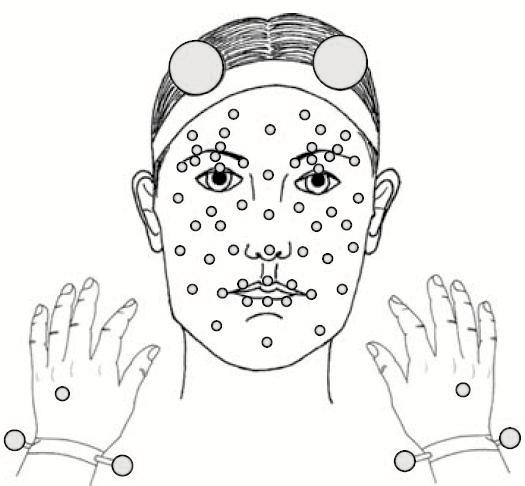
\includegraphics[width=0.32\textwidth]{figures/Ch4/IEMOCAP_marker_positions.jpg}
\caption{Marker Layout used in recording for IEMOCAP dataset~\cite{Busso08}.}
\label{fig_marker_layout}
\end{figure}

The released version of the dataset contains approximately 12 hours of audiovisual data, including video, speech, motion capture of face, text transcriptions. It consists of dyadic sessions (5 sessions with 2 subjects each), where actors perform improvised hypothetical scenarios and selected emotional scripts, specifically selected to elicit emotional expressions (happiness, sadness, anger, frustration, and neutral state).

During each interaction, only one of the two actors was motion captured at a time while performing improvised and scripted dialogs. Each dialog consists of almost 25 utterances/turns of each actor, where an utterance is a sentence or similar period during which one actor talks continuously. The dataset contains ten thousand and thirty nine utterances where each utterance consists of almost 11.4 words with an average duration of 4.5 seconds. 

Within each dialog, each utterance of the two actors was annotated by three independent human evaluators into categorical labels (neutral, happiness, anger, sadness, surprise, disgust, fear, frustration, and excitement) as well as psychological data about emotion intensity (valence, activation, and dominance). 

These two approaches cover the categorical as well as continuous attributes of emotional representation. The emotion content of the dataset was annotated by the evaluators into categorical labels using the ANVIL tool~\cite{Kipp2001Anvil}, after sequentially watching the videos. In this way, the evaluators had information from audio and video channels as well as previous utterances in the dialog for assessing the emotional content of each utterance. It was assumed that within an utterance, there is no emotion transition (e.g., from happy to excited), however, the evaluators were allowed to select more than one emotion category to describe mixtures/blends of emotions, which are more common in natural communication. The estimated confusion matrix between the assigned categorical labels shows that there is an overlap between happiness and excitement as well as anger and frustration. Neutral, disgust, and anger are often get confused with frustration. Also, sadness is often confused with frustration and neutral.

The evaluation-level limitation of the selected dataset is associated with its utterance-based annotation technique. Assuming the emotional content did not change much within an utterance (duration $\approx$ 4.5 seconds), the same label (or mixture of labels) was assigned to each frame in that utterance. The `silent' frames and those containing sounds of active listening like `mmhh' were not annotated at all. Another problem of the chosen dataset is that the human evaluators were sometimes inconsistent in labelling the data, since each one of them perceived and evaluated the emotions associated to an utterance in his own way. Due to the subjective nature of emotions, the inter-evaluator inconsistency is a common problem of all emotion datasets.

\subsubsection{Data Preprocessing}
\label{sec_data_preprocessing}

We used the locations of the marker points in 3D as the basis of our analysis, and chose $5,000$ frames of each of five emotions (happiness, excitement, anger, frustration, and sadness) and neutral state for each of the ten actors to form a training set of $300,000$ frames. It should be noted that the marker points were already aligned to make the nose marker at the center of each frame that removed any translation effects. The rotational effects were compensated by multiplying each frame by a rotational matrix. For details about markers alignment, refer to~\cite{Busso08}. 

Each utterance was labelled by the three expert human evaluators in terms of discrete categories as well as emotion attributes (valence and activation). For the training set, we took frames from the utterances where all three experts agreed. We used six emotions rather than the full nine as for the missing emotions (disgust, surprise, and fear) there was insufficient data, sometimes as little as $2,000$ frames in total. Out of the six selected emotions, two (frustration and excitement) are the candidate basic emotions~\cite{ortony1990s, ekman1999basic}. The selection of the testing set would be described in Section~\ref{sec_shape_models} depending on the type of model (dependent or independent) used for training. For the testing set, there was no such condition of agreement by all three experts while choosing the frames.

Each frame of the dataset contains the motion capture information of 61 markers in 3 dimensions, so the training data was of size $300,000 \times 183$ dimensions. We reduced the dimensionality of the data for each frame in three ways:

\begin{enumerate}
\item Markers not on the face (such as the head and hands) were excluded.
\item Markers that did not move significantly (such as eyelids and nose) were removed. 
\item Sets of markers that moved together (such as, points on the chin and forehead) were replaced by a single point at the centre of the set.
\end{enumerate}

\begin{figure*}[ht!]
\begin{center}
		\subfloat[rotation: $0\degree$]
		{ 
		\centering
		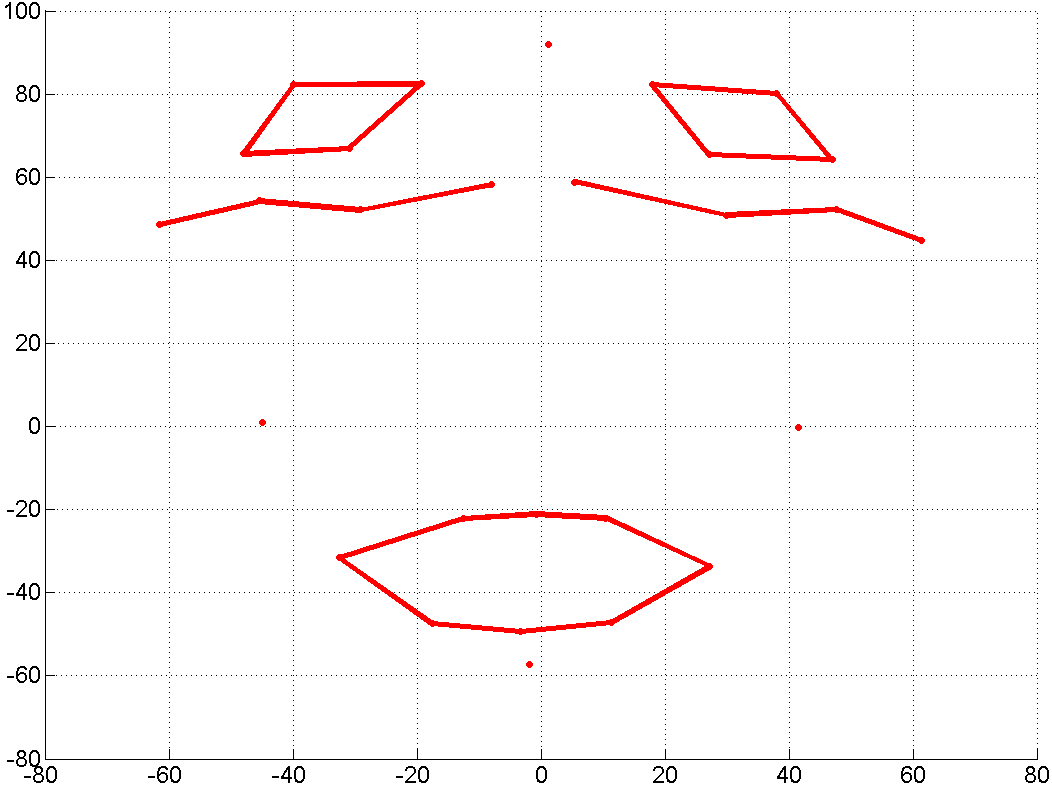
\includegraphics[width=0.2\textwidth]	{figures/Ch5/full_face/0,0.png}
		}
		\subfloat[rotation: $30\degree$]
		{ 
		\centering
		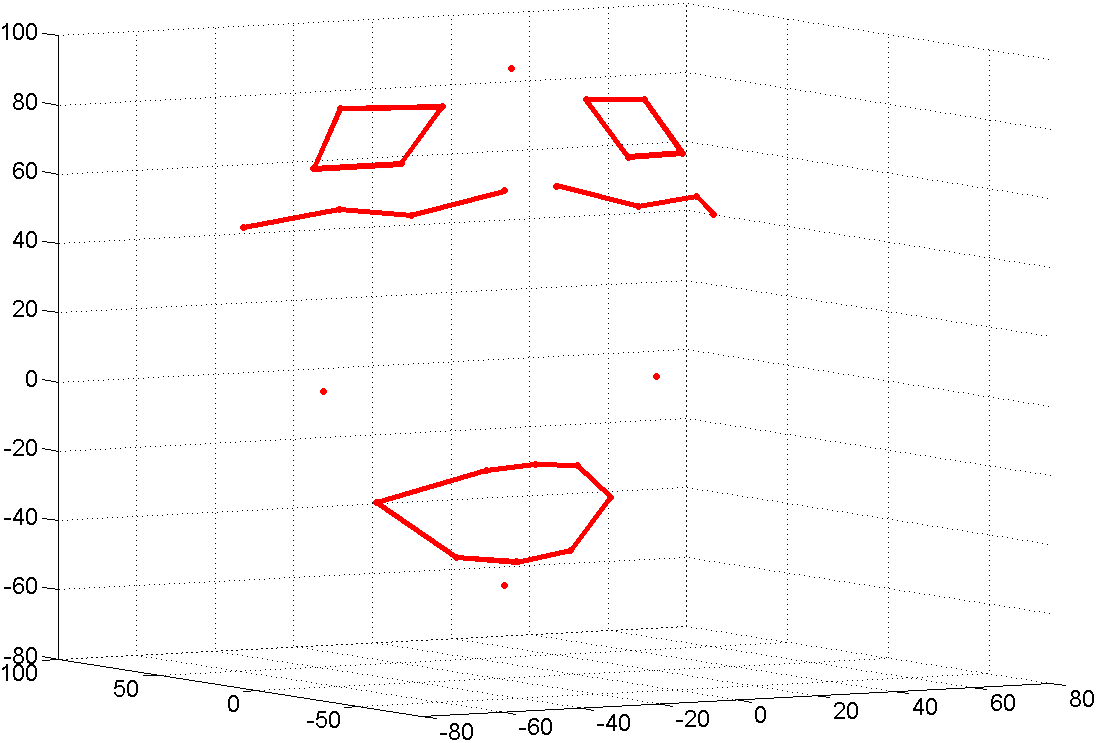
\includegraphics[width=0.2\textwidth] 	{figures/Ch5/full_face/-30,6.png}
		}
		\subfloat[rotation: $60\degree$]
		{ 
		\centering
		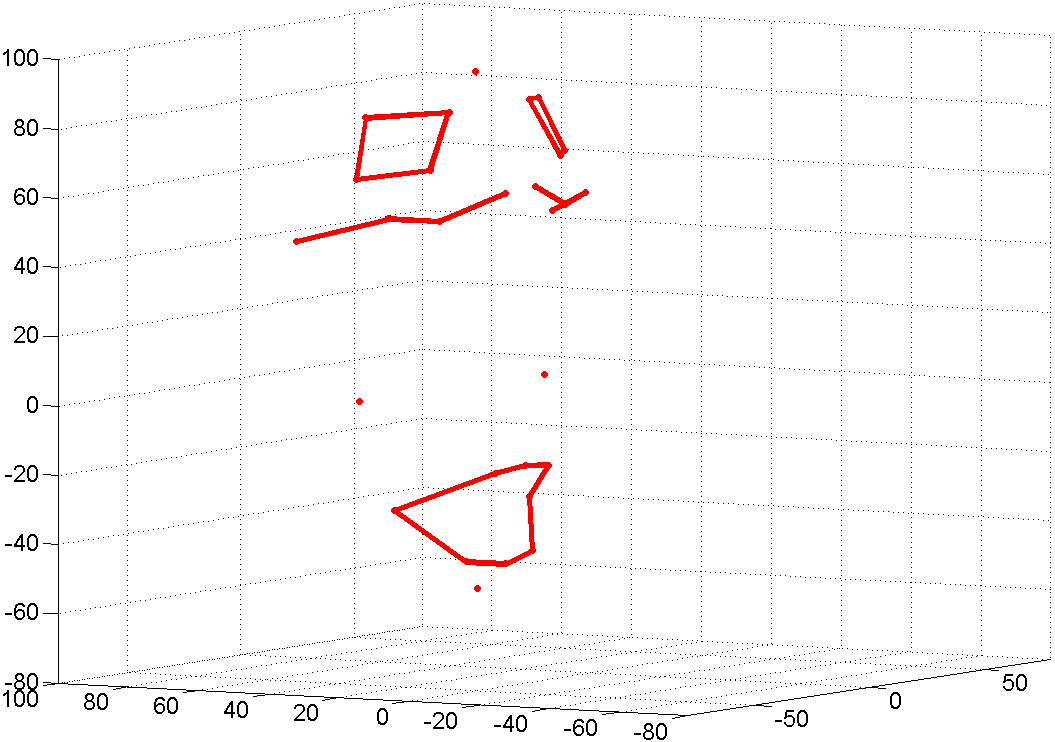
\includegraphics[width=0.2\textwidth] 	{figures/Ch5/full_face/-60,6.png}
		}
		\subfloat[rotation: $90\degree$]
		{ 
		\centering
		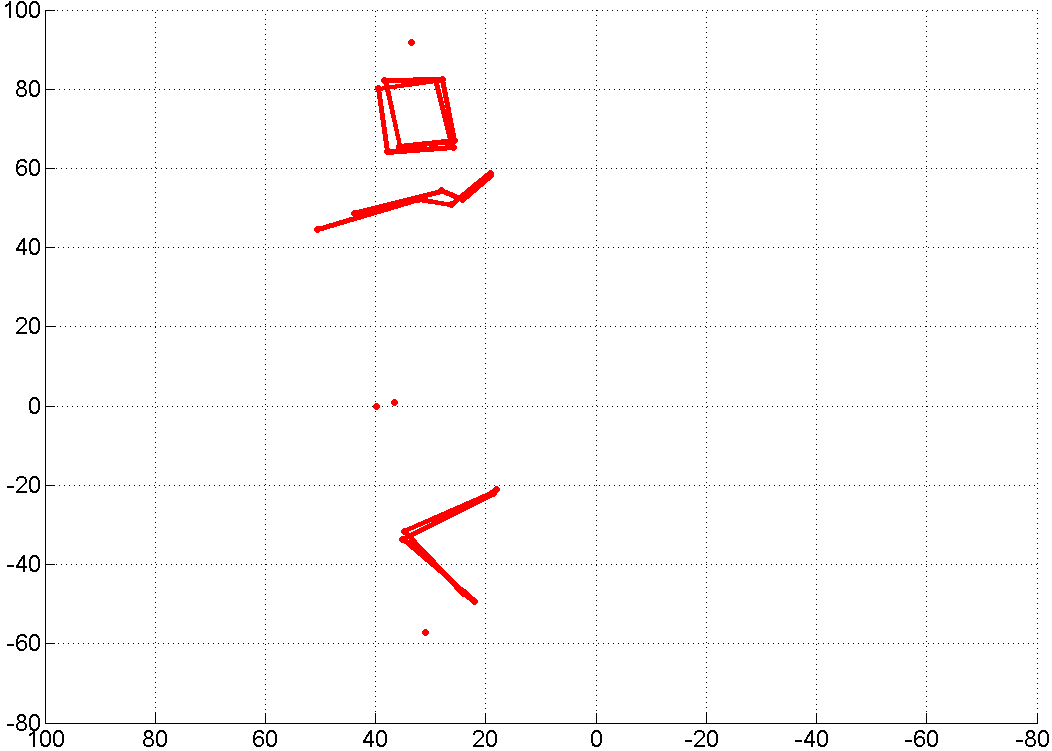
\includegraphics[width=0.2\textwidth] 	{figures/Ch5/full_face/-90,0.png}
		}
\caption{The 28 marker points in 3D used for emotion recognition and analysis.}
\label{fig_markers_3D}
\end{center}
\end{figure*}


As a result of these simplifications each emotion frame is represented by 28 markers points covering the forehead, eyebrows, eyes, cheeks, lips, and chin (Fig.~\ref{fig_markers_3D}). The location of marker points are in 3D, making it an 84D vector.

\subsection{Shape Models}
\label{sec_shape_models}

Based on the data from IEMOCAP we had sets of facial points with an associated emotion label. As described in Section~\ref{sec_data_preprocessing}, we are using the 3D locations of 28 marker points on the face for emotion recognition and analysis. We then develop two types of models: a model of only one actor at a time that we called the \textbf{speaker-dependent model}, and a model of nine out the ten actors that we called the \textbf{speaker-independent model}. 

The \textbf{speaker-dependent model} is trained on $5000$ frames of each emotion of one actor only to form a training set of $30,000$ frames. We then used principal component analysis (PCA) to develop a face model of the given training set based on the method described in~\cite{ayesha hakim shape model paper}. We noticed that the first 7 PCs covered $93\%$ of the total variation of the training data out of which the first PC, which covers almost $50\%$ of the total variation, was describing the upward and downward movement of the mouth points. This movement of lips was experimentally shown to be highly correlated with talking~\cite{ayesha hakim shape models}, which is not directly connected with emotion recognition, and not much else, and so we discarded the first PC. Consequently, we chose to use six PCs (2-7) of the face model for our analysis. For details about the effects of each principal component on the mean face, refer to~\cite{ayesha hakim shape models}.

We transformed the training data into the 6-D space of the selected six principal components. Each datapoint was then labelled with the majority vote of the three human experts, so that the training set consists of 30,000 points, each labelled with one of six emotions in the 6-D space. 

To evaluate the speaker-dependent face model, we chose the continuous testing frames of the same actor on which the model was trained. That was the ideal situation as there was only one face involved leading to no speaker variability and the first PC correlated to talking was removed leading to no lexical variability. For classification of a test frame, it was transformed into the 6-D space of the dependent face model. We then computed the Mahalanobis distance between the test frame and the six emotion clusters. In this way, we get a set of six distances; one for each emotion in the model space. We use these distances to map the emotion into the activation-evaluation space~\ref{sec_mapping}.

The \textbf{speaker-independent model}  is trained on $5000$ frames of each emotion of nine actors to form a training set of $270,000$ frames. We then again used PCA to develop a face model of the given training set and noticed that the first $15$ PCs covered $90\%$ of the total variation of the training data. Unlike speaker-dependent model, the first PC was not describing talking movements rather was related to the face variations of nine different speakers. However, the speaker variation was not too well defined in the first few PCs to discard. 

To evaluate the speaker-independent face model, we chose the continuous testing frames of one of the ten actors that was not included in the training set. For classification of a test frame, it was transformed into the 11D space of the independent face model. We then computed the Mahalanobis distance between the test frame and the six emotion clusters to get a set of six distances; one for each emotion in the model space. We use these distances to map the emotion into the activation-evaluation space~\ref{sec_mapping}.

%Reference-based Speaker Normalisation
\subsubsection{Speaker Normalisation}
The speaker variability in the \textbf{speaker-independent model} is removed by reference-based speaker normalisation that is quite similar to the technique used in~\cite{ACTORIZING SPEAKER, LEXICAL AND EMOTIONAL VARIABILITIES OBSERVED IN FACIAL EXPRESSIONS}. 

%edit it
The neutral interaction of the female subject in the first session of the database is selected as the reference speaker. The technique is about matching the first and second order statistics of facial points movements across all the speakers with respect to the reference speaker. The markers of other speakers are mapped into the markers' space of the reference speaker. Equation~\ref{eq_normalisation} describes this speaker normalization technique. The $i^{th}$ marker of the speaker s in the direction $d \in {X,Y,Z}, (m_{i,d}^{s})$, is transformed to match the reference speaker $(ref)$, where $\mu$ and $\sigma$ are the mean and standard deviation of the markers.
\begin{equation}
m_{i,d}^{s'}=(m_{i,d}^{s'}-\mu_{i,d}^{s'}) \times \frac{\sigma_{i,d}^{ref}}{\sigma_{i,d}^{s}} + \mu_{i,d}^{ref}
\label{eq_normalisation}
\end{equation}

%add equation

After speaker normalisation, we retrain the \textbf{speaker-dependent model} on the normalised  $30,000$ frames containing all emotions of one actor only and used PCA to develop a normalised face model of that actor. We repeated the same experiment on the normalised $270,000$ frames of all excluding one speaker to get a normalised \textbf{speaker-independent model}. Section~\ref{sec_results} shows the comparison of all face models: speaker-dependent face model, speaker-independent face model, normalised speaker-dependent face model, and normalised speaker-independent face model.

\subsubsection{Classification}

For classification based on each face model separately, we replaced each cluster (i.e., set of points labelled as one emotion) with the mean of that set, and also computed the covariance matrix (spread) of the data. We therefore ended up with six datapoints representing the mean of each set and an associated covariance matrix. 

For classification of a test frame, it was transformed into the transformed space of each model separately. We then computed the Mahalanobis distance between the test frame and each of the six emotion clusters. In this way, we got set of six distances; one for each emotion in each model space.
We then labelled the test point with the label of the cluster that it is closest to. The Mahalanobis distance not only uses the mean, but also takes into account the spread of the data to compute a distance. It is formulated as:

%It is named after the person who described it in 1936, and is forumlated as:
\begin{center}
$ D_{M}(\mathbf{x}) =\sqrt{(\mathbf{x}-\mathbf{\mu})^{T}\Sigma^{-1}(\mathbf{x}-\mathbf{\mu})} $
\end{center}

\noindent where $\mathbf{x}$ is the (4D) column vector of the test frame, $\mathbf{\mu}$ is a column vector of the mean and $\Sigma$ is the $4 \times 4$ covariance matrix for an emotion. If the covariance matrix is set to the identity matrix, then the Mahalanobis distance reduces to the Euclidean distance~\cite{Mahal1936, Marsland09}.

Computing the Mahalanobis distance is a computationally expensive process which calculates the covariance matrix and then its inverse. For efficient computation, we have used Matlab's \textit{mahal} from the Statistics toolbox to compute the Mahalanobis distance of each frame to each of the six emotion clusters. 

\subsection{Mapping emotions into the activation-evaluation space}
\label{sec_mapping}

%We have calculated the Mahalanobis distance of each test frame to each of the six basic emotions using the shape models (using the method described in Section~\ref{sec_shape_models}). 
There are two steps required to map the representation of the facial points of an image frame into the activation-evaluation space: represent the basic emotions as points within that space, and then position each frame (using the six distances to the basic emotions). The first of these steps uses the training data, which is assumed to represent each of the six basic emotions (all three experts agreed on their labels), while the second uses the testing data. We used the same technique to calculate the position of mean emotions and test frames on the emotion-space.

%calculation of mean emotions
For each of the four face models, we calculated the position of the mean emotions separately based on the respective training data set. For each training set separately, we developed one shape model and calculated the distance of each frame from each of the five emotion clusters($\beta_{ang}, \beta_{fru}, \beta_{hap}, \beta_{exc}, \beta_{sad}$) and the neutral state ($\beta_{neu}$). 

Each frame is assumed to be a combination of the basic emotions, and so we needed to calculate the weighted average of basic emotions, where the weights correspond to the classification confidence of test frames for each basic emotion. We calculated the weight of each emotion and the neutral state as follows,

\begin{equation}
\gamma_{j}=\left(\frac{\beta_{j}}{\sum \limits_{i=1}^6 \beta_{i}} \right) ^{-1}
\label{eq_weights}
\end{equation}

where $j$ is the number of emotions and the neutral state.

To calculate the weighted average of basic emotions for each frame, we modelled the distribution of each basic emotion as a von Mises distribution and constructed a mixture model of them. This is described in Section~\ref{sec_von_Mises}.

To plot the mean of each emotion in the emotion-space, we calculated the x-coordinates and y-coordinates for each frame as follows:

\begin{equation}
\bar{X}=\frac{1}{n}\sum \limits_{i=1}^n x_{i}, \; \; \; \bar{Y}=\frac{1}{n}\sum \limits_{i=1}^n y_{i}
\end{equation}
where $n$ is the number of frames of each emotion, $x_{i}$ and $y_{i}$ would be calculated using the mixture of von mises distribution as discussed in Section~\ref{sec_von_Mises}.

It should be something like this. or should mention mixture model here:

\begin{equation}
\begin{array}{ll} 
\bar{X}=\sum \limits_{i=1}^j \gamma_{i} \times cos(\theta_{i}) \\
\bar{Y}=\sum \limits_{i=1}^j \gamma_{i} \times sin(\theta_{i})
\end{array}
\end{equation}

where $j$ is the number of emotions and the neutral state.

We calculated the mean magnitude of the resultant vector for each of the six emotions separately as follows,

\begin{equation}
\label{eq:meanint}
\bar{R}^{2}=\bar{X}^{2} + \bar{Y}^{2}
\end{equation}

The mean of $\bar{R}$ corresponds to the mean intensity of each emotion in the activation-evaluation space.

To calculate average angles it is not appropriate to use the linear statistical mean average due to the reasons discussed in Section~\ref{sec_analysis}. Therefore, we chose to calculate the geometric mean to get the angular position of each of the mean emotions in the activation-evaluation space. The computation of the mean direction is as follows:

\begin{equation}
\label{eq:meandir}
\mu= \left\{ \begin{array}{ll}
\tan^{-1}(\bar{A}/\bar{V}) & \bar{A}>0, \bar{V}>0 \\ 
\tan^{-1}(\bar{A}/\bar{V})+\pi & \bar{V}<0 \\ 
\tan^{-1}(\bar{A}/\bar{V})+2\pi & \bar{A}<0, \bar{V}>0
\end{array}\right.
\end{equation}

$\mu$ is the mean direction and $\bar{R}$ corresponds to the mean intensity of emotions and neutral state in the activation-evaluation space. This gave us locations for the basic emotions and the neutral state. The location of each test frame is also calculated by the using equation~\ref{eq:meanint} and~\ref{eq:meandir}.

\subsubsection{von Mises Mixture Model}
\label{sec_von_Mises}

A circular variable $\theta$ is said to have a von Mises distribution if the probability density function is given by:
\begin{equation}
m(\theta;K,\mu) = \frac {1}{2 \pi I_{0} (K)} e^{[K\cos (\theta - \mu)]}
\end{equation}
where $0 \leq \theta < 2 \pi$, $K > 0$ and $0\leq\mu<2\pi$.

The parameter $\mu$ is the mean direction and $K$ is the concentration parameter, which is analogous to the (inverse) variance: the density at the mode depends on $e^{2K}$ and the larger the value of $K$, the greater is the clustering around the mode. The distribution is uni-modal and symmetric about $\mu$. $I_{0}(K)$ is a normaliser to turn this into a probability density function and consists of a modified Bessel function of the first kind of order zero~\cite{chang1996computation}:

\begin{equation}
I_{0}(K)= \sum \limits_{r=0}^\infty \frac{1}{r!^{2}} \left(\frac{1}{2}(K)^{2r}\right)
\end{equation}

Although each emotion class is uni-modal, we cannot fit one von Mises distribution to the full data as it is the mixture of six different emotion classes. Such multi-modal distributions may be regarded as mixtures of uni-modal distributions~\cite{mardia1972statistics}. We used a finite mixture model of six uni-modal von Mises distributions, given by: 

\begin{equation}
M=\sum \limits_{j=1}^6 \gamma_{j}m_{j}(\theta)
\end{equation}

where $\gamma_{j}$ are non-negative weights that sum to one. We have already calculated the mean direction $(\mu_j)$ of each of the six reference emotions in the space using Eq.~(\ref{eq:meandir}), and the methods of estimating $K_{j}$ and $\gamma_{j}$ are described in the following section.

\subsubsection{Estimating the Parameters of the Mixture Model}
\label{sec_est_para}
There are several ways to estimate the parameters on which the mixture model depends~\cite{mardia1972statistics}. We have used the usual maximum likelihood estimate for $K_{j}$. However, the weights $\gamma_{j}$ of each emotion model are estimated by using the distances to the six emotions calculated by the shape models.

\paragraph{Estimating the concentration parameter}
\label{sec_est_kappa}
The concentration parameter $K_{j}$ is estimated by using the Fisher equation~\cite{fisher1995statistical}:
\begin{equation}
\label{eq:kappa}
\hat{K}_{ML}=\left\{ \begin{array}{ll}
2\bar{R}+\bar{R}^{3}+5\bar{R}^{5}/6 	&	 \bar{R} < 0.53 \\ 
-0.4+1.39\bar{R}+0.43/(1-\bar{R}) 		&	 0.53 \leq \bar{R} < 0.85 \\ 
1/(\bar{R}^{3}-4\bar{R}^{2}+3\bar{R}) 	&	 \bar{R} \geq 0.85 \\ 
\end{array}\right.
\end{equation}
$\hat{K}_{ML}$ may be biased if the sample size ($n$) and $\bar{R}$ are small (specially when $\bar{R}<0.45$). For this reason, if $n \leq 15$, the following estimate is to be preferred:
\begin{equation}
\hat{K}=\left\{ \begin{array}{ll}
\max(\hat{K}_{ML}-2(n\hat{K}_{ML})^{-1},0) 	&	 \hat{K}_{ML} < 2 \\ 
(n-1)^{3}\hat{K}_{ML}/(n^{3}+n) 				&	 \hat{K}_{ML} \geq 2
\end{array}\right.
\end{equation}

\noindent This is a standard approach for estimating the concentration parameter~\cite{fisher1995statistical, mardia1972statistics}.

\paragraph{Estimating the weights}
\label{sec_est_weight}
We have already calculated the Mahalanobis distance of each test frame to each of the six basic emotions using the shape models. We want to position each test frame in activation-evaluation space using the positions of the basic emotions. However, the Mahalanobis distance is an unsigned quantity and so we do not know the direction between the test frame and the mean of each of the clusters of basic emotions. Since we have assumed that each emotion lies along a radial line in the activation-evaluation space we want to compute the intensity of each of the basic emotions as a component of the complex emotion. We did this starting at the position of the basic emotion and then by applying a simple rule to move along that radial line: if the distance of the test frame from neutral is less than the mean of a particular emotion, then the distance of the test frame from that emotion should be towards neutral i.e., its intensity decreases and comes close to neutral and vice-versa. We convert these distances to weights $(\gamma_{j})$ using equation~\ref{eq_weights}.

\section{Results}
\label{sec_results}

% Edit Table mean emotions

\begin{table*}[tp!]
\caption{Mean intensity of five emotions and neutral state estimated using dependent and independent models both with and without performing speaker-normalisation.}
\centering
\begin{tabular}{|p{1.5cm}|p{1.5cm}|p{1.5cm}|p{1.5cm}|>{\centering\arraybackslash}p{2.5cm}| >{\centering\arraybackslash}p{3.2cm}|>{\centering\arraybackslash}p{2.5cm}|}
\hline
\multicolumn{7}{|c|}{\textbf{Without Normalisation}} \\
\hline
 & Neutral &  Anger & Frustration & Happiness & Excitement & Sadness  \\
\hline
Dependent Model & 0.3095 &  0.5167 & 0.6066 & 0.4168 & 0.6152 & 0.4968  \\
\hline
Independent Model & 0.1286 & 0.2698 &  0.1809 & 0.2704 & 0.2278 & 0.1663  \\
\hline
\multicolumn{7}{|c|}{\textbf{With Reference-based Speaker Normalisation}} \\
\hline
Dependent Model & 0.3095 &  0.5167 & 0.6066 & 0.4168 & 0.6152 & 0.4968  \\
\hline
Independent Model & 0.1693 & 0.3325 &  0.2759 & 0.3523 & 0.3628 & 0.2414  \\
\hline
\end{tabular}
\label{table_mean_emotions}
\end{table*}

%Plot instead of Table?

Table~\ref{table_mean_emotions} lists the mean locations of the five emotions and neutral state in the activation-evaluation space based on different training sets. For the training data of the first speaker only, the mean intensity of five emotions and neutral state remain same with and without normalisation. For the training data of all speakers together, the mean intensity of emotions decreases without normalisation caused by the speaker variation  leading to confused emotion recognition. The mean intensity increases after reference-based speaker normalisation.

We observed that the estimated directions of each emotion based on training data are quite close to those specified by Whissell in~\cite{Whissell89}, except that of neutral state.  According to the values listed by Whissell, neutral lies close to the centre of circle that corresponds to both valence and activation close to zero. In our data, since the direction of neutral is calculated as weighted average of all emotions its more inclined towards anger/frustration. One reason is that there are more emotions on the side of negative emotions than the positive emotions. Other reason is based on the fact that mostly the human evaluators misinterpreted neutral as frustration or sadness. This direction of neutral state does not effect the position of other emotions because the neutral state represents the `no-emotion' state whose position should be uncorrelated with that of all emotional states.

%-----------------------

Based on these positions for the basic emotions we were now able to compute the parameters of the mixture model and test it using initially single utterances with only one labelled emotion, and then full dialogs with several emotion transitions. We use the valence and activation values assigned to each utterance by three human experts to estimate the ground truth direction and intensity of emotion associated with that utterance, which we can compare to our results~\cite{ayesha von mises}. 

\begin{figure*}[tp!]
\begin{center}
		\subfloat[]
		{ 
		\centering
		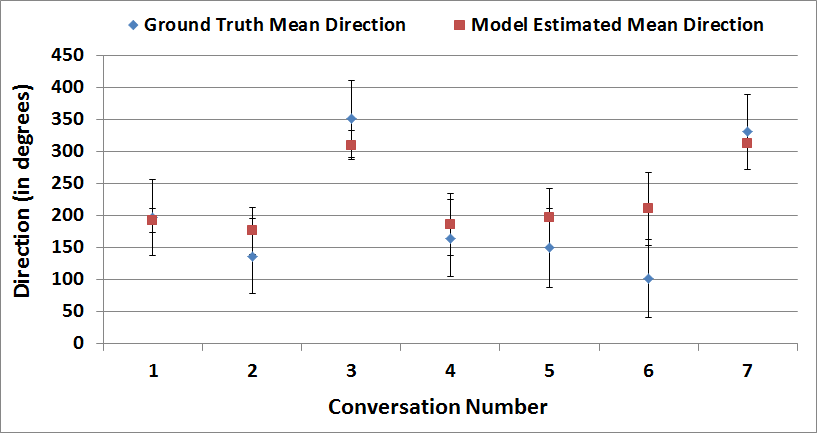
\includegraphics[width=0.5\textwidth]{figures/Ch6/comparison_dir_updated_2.png}
		}
		\subfloat[]
		{ 
		\centering
		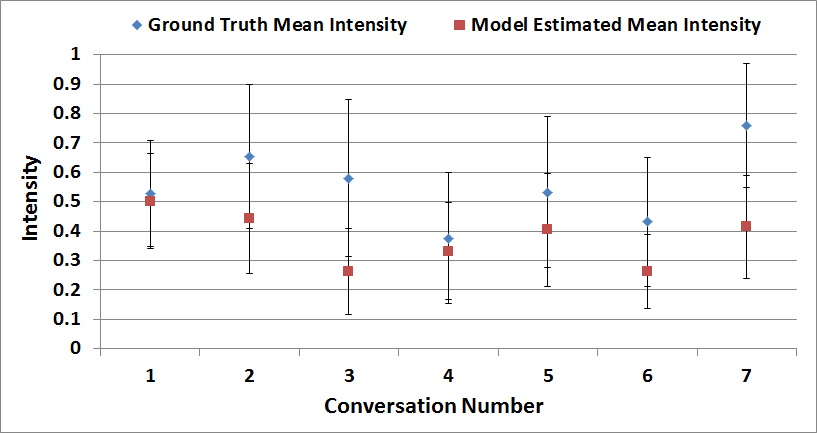
\includegraphics[width=0.5\textwidth]{figures/Ch6/comparison_int_updated_2.png}
		}
\end{center}
		\caption{The test of fit for (a) the mean ground truth \textit{directions} and those estimated by the mixture model (b) the mean ground truth \textit{intensities} and those estimated by the mixture model, for each of the seven conversations in the test set. Lines mark one standard deviation.}
		\label{fig_comparison}
\end{figure*}

In order to test the goodness of fit of two sample distributions (ground truth and model estimation), we also used Kuiper's test, which is a circular analogue of the Kolmogorov-Smirnov test~\cite{watson1982circular, mardia1972statistics}. Let $F(\theta)$ denote the continuous cumulative distribution function (cdf) of each of the emotions in the mixture model separately and $S_{n}(\theta)$ be the ground truth cdf (referred to as the empirical cdf). The Kuiper's statistic is defined as,

\begin{equation}
V_{n}=D_{n}^{+}+D_{n}^{-}
\label{eq_kstatistic}
\end{equation}

\noindent where

\begin{equation}
D_{n}^{+}=\max[S_{n}(\theta)-F(\theta)], \;\;\;\; D_{n}^{-}=\max[F(\theta)-S_{n}(\theta)]
\label{eq_deviation}
\end{equation}

$D_{n}^{+}$ and $D_{n}^{-}$ are the discrepancy statistics, where $D_{n}^{+}$ is the maximum vertical distance of $S_{n}(\theta)$ from $F(\theta)$ when the distance is measured above $F(\theta)$, while $D_{n}^{-}$ is the maximum distance measured below $F(\theta)$. Both statistics $D_{n}^{+}$ and $D_{n}^{-}$ depend on the choice of zero direction, but their sum ($V_{n}$) is invariant under rotation. This makes the Kuiper's statistic equally sensitive at the median as well as at the tails~\cite{kuiper1960tests, mardia1972statistics}.

Fig.~\ref{fig_kuiper} shows the model estimated cdf of each of the emotions in the mixture model separately and the empirical cdf for the first dialog in the testing set. It can be seen that the model estimated cdf for anger (Fig.~\ref{fig_kuiper}(a)) as well as that of frustration (Fig.~\ref{fig_kuiper}(b)) fits the empirical cdf well. However, the cdfs for happiness (Fig.~\ref{fig_kuiper}(c)), excitement (Fig.~\ref{fig_kuiper}(d)), and sadness (Fig.~\ref{fig_kuiper}(e)) show quite high deviation from the empirical cdf. This suggests that the empirical distribution and the model estimated distributions of anger as well as frustration are not statistically different. On the basis of this, we may say that the first conversation in the testing set is an angry/frustrated conversation.

\begin{figure*}[htp!]
\begin{center}
		\subfloat[cdf of anger]
		{ 
		\centering
		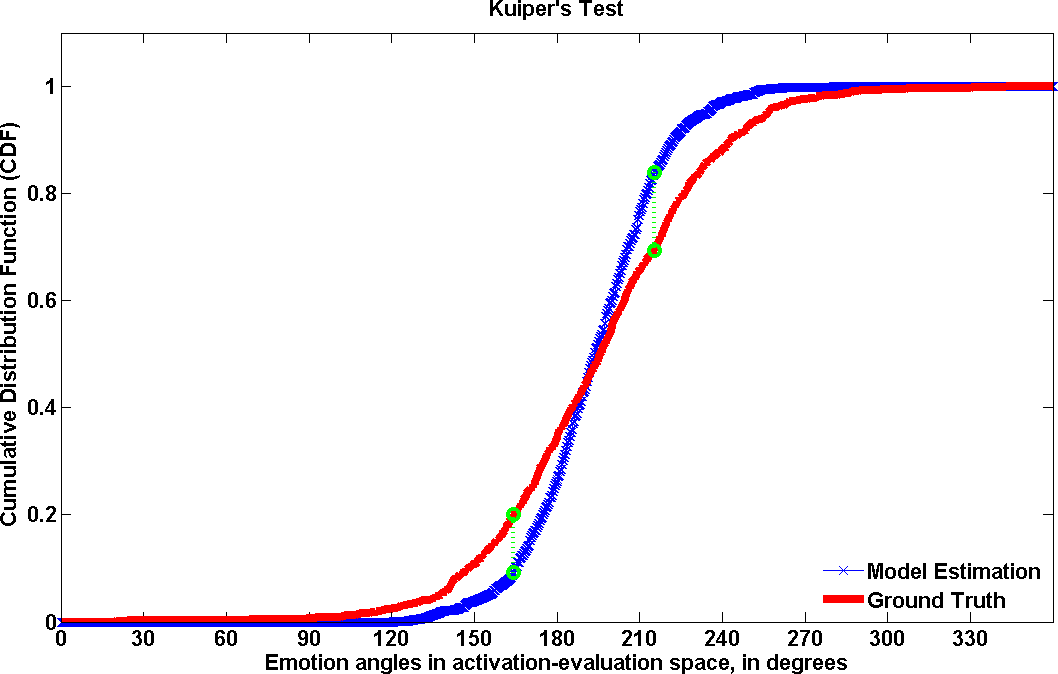
\includegraphics[width=0.3\textwidth]{figures/Ch6/separate_cdfs/cdf_with_ang_up1.png}
		}
		\subfloat[cdf of frustration]
		{ 
		\centering
		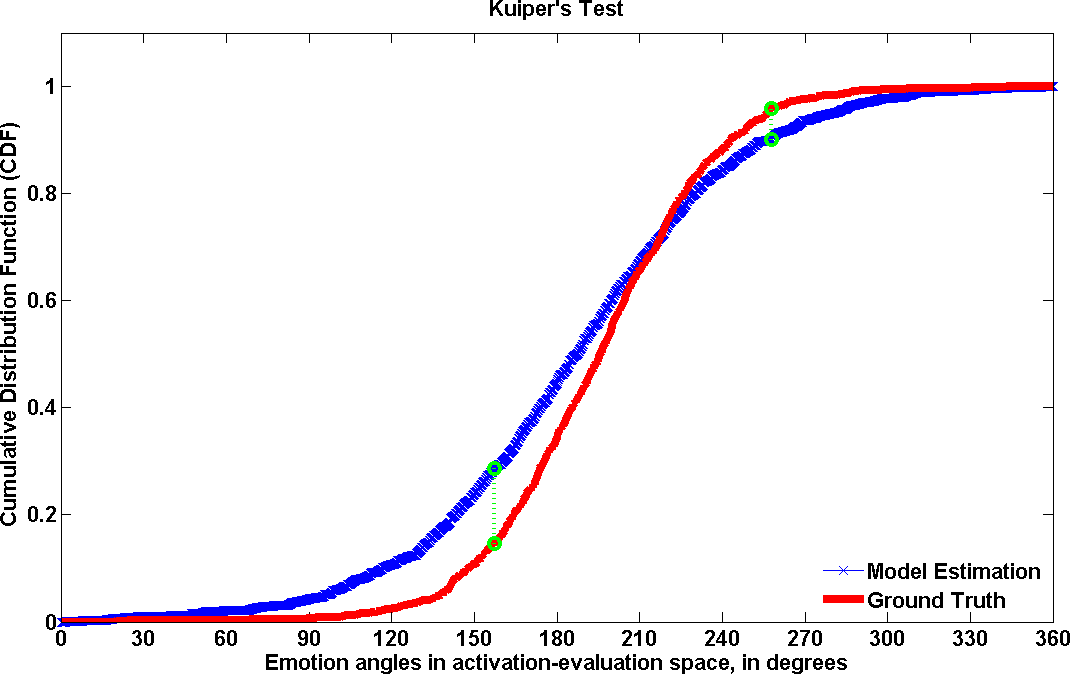
\includegraphics[width=0.3\textwidth]{figures/Ch6/separate_cdfs/cdf_with_fru_up1.png}
		}
		\subfloat[cdf of sadness]
		{ 
		\centering
		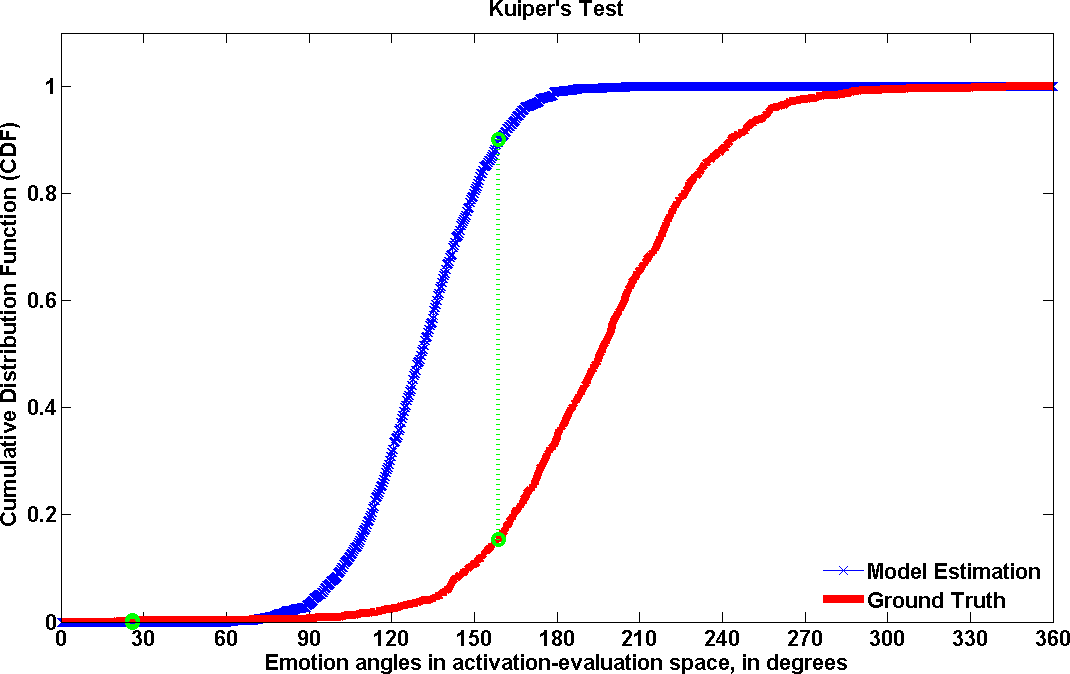
\includegraphics[width=0.3\textwidth]{figures/Ch6/separate_cdfs/cdf_with_sad_up1.png}
		}
		\\
		\subfloat[cdf of happiness]
		{ 
		\centering
		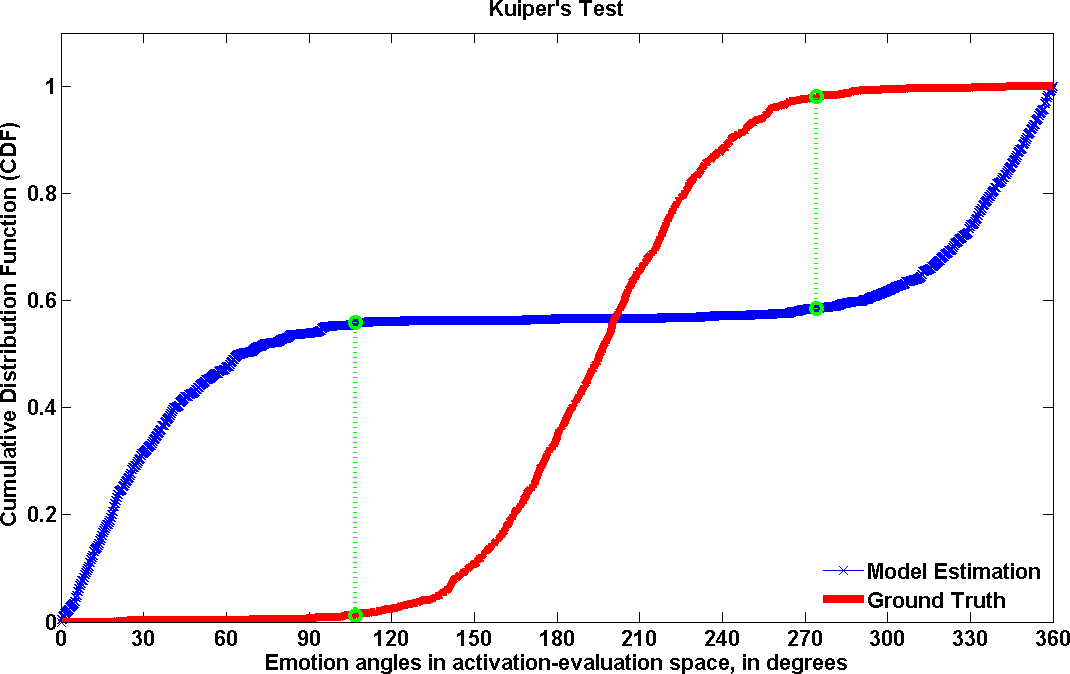
\includegraphics[width=0.3\textwidth]{figures/Ch6/separate_cdfs/cdf_with_hap_up1.png}
		}
		\subfloat[cdf of excitement]
		{ 
		\centering
		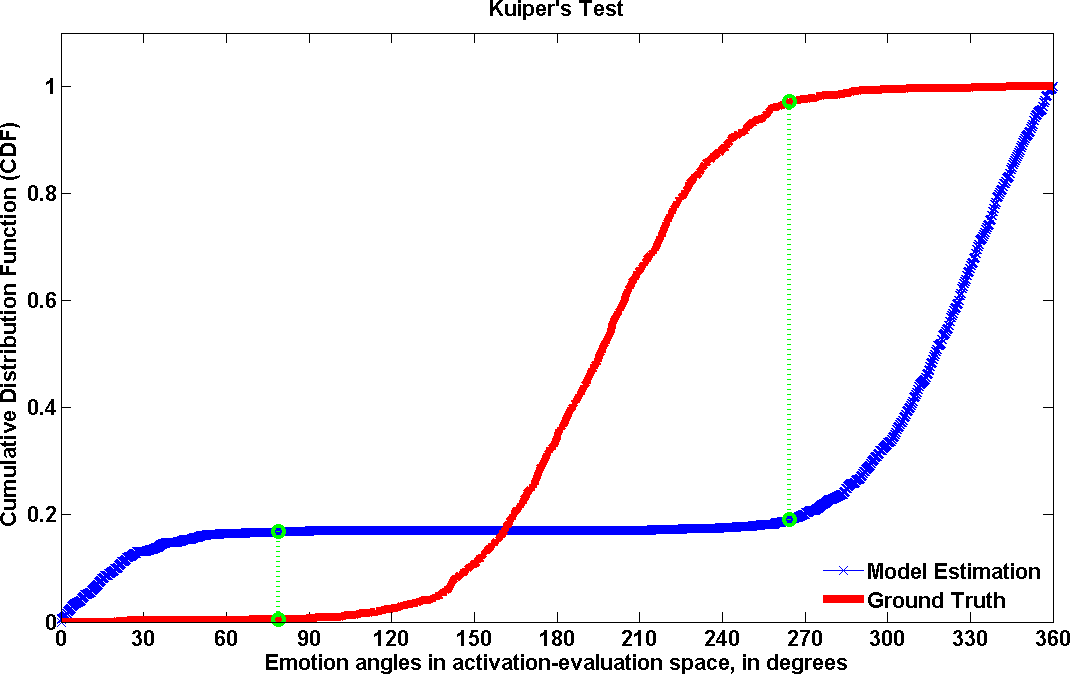
\includegraphics[width=0.3\textwidth]{figures/Ch6/separate_cdfs/cdf_with_exc_up1.png}
		}
\end{center}
		\caption{Illustration of the Kuiper's statistic. Blue line is model estimated CDF of (a) anger, (b) frustration, (c) sadness, (d) happiness, and (e) excitement, red line is an empirical CDF of the first conversation in the testing set, and the green line is the Kuiper's statistic.}
		\label{fig_kuiper}
\end{figure*}

Figs.~\ref{fig_comparison} and~\ref{fig_kuiper} show that the proposed mixture model fits the data well, despite the underlying problems with the ground truth labelling (that is, the fact that there is only one label associated with each utterance, which lasts for many frames while the model estimates the values for each frame). Furthermore, all `silent' frames are unlabelled in the conversations, while the model estimates the values for those frames as well.  The intensity values do not fit as well as the directions because the small number of samples leads to high concentration around the mean as compared to the large number of frames in the testing set.

\begin{figure*}[!htp]
\begin{center}
\subfloat[Full dialog, Ses01F$\_$impro01, continuous frames during emotion transition without normalisation. Dependent Model.]
{
\centering
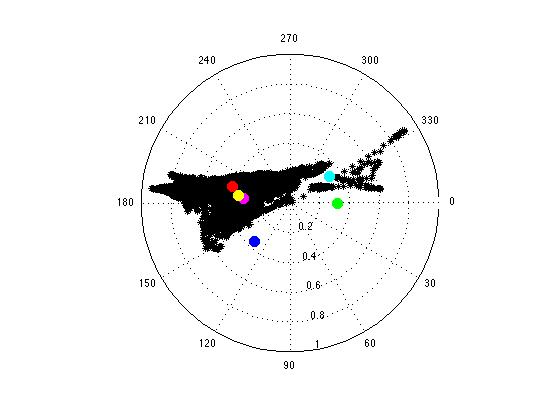
\includegraphics[width=0.5\textwidth]{figures/new_results/without_normalisation/Ses01F_impro01_actor1_full_map_not_0_1.jpg}
}
%\\
\subfloat[Full dialog, Ses01F$\_$impro01, continuous frames during emotion transition without normalisation. Independent Model.]
{
\centering
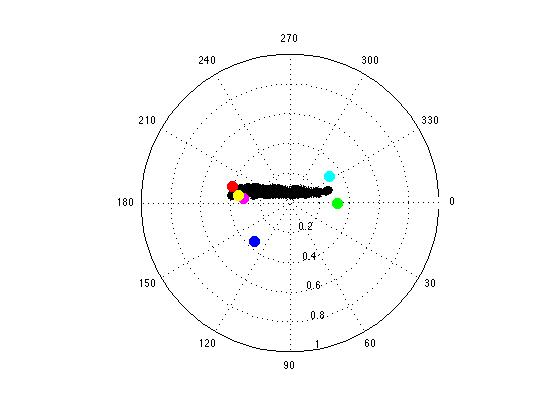
\includegraphics[width=0.5\textwidth]{figures/new_results/without_normalisation/Ses01F_impro01_actor2_10_full_map_not_0_1.jpg}
}
\\
\subfloat[Full dialog, Ses01F$\_$impro01, continuous frames during emotion transition with normalisation. Dependent Model.]
{
\centering
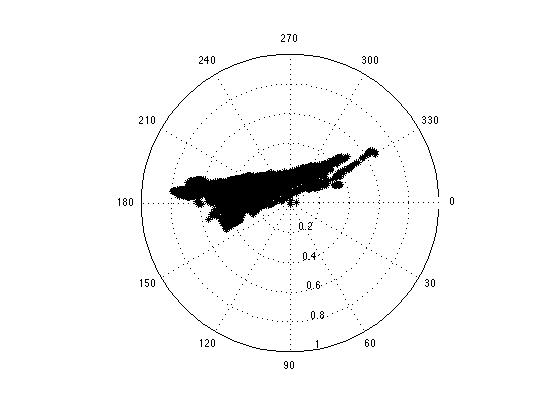
\includegraphics[width=0.5\textwidth]
{figures/new_results/with_ref_normalisation/Ses01F_impro01_actor1_full_map_not_0_1_nomeans.jpg}
}
\subfloat[Full dialog, Ses01F$\_$impro01, continuous frames during emotion transition with normalisation. Independent Model.]
{
\centering
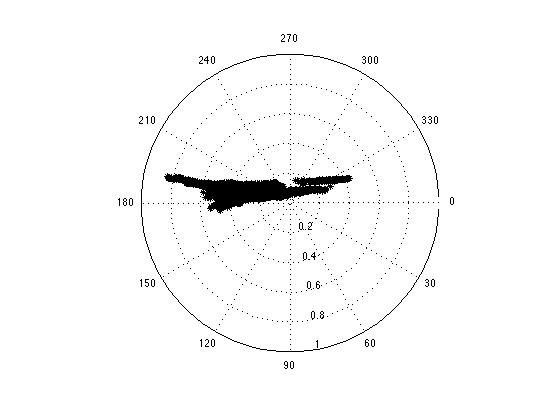
\includegraphics[width=0.5\textwidth]{figures/new_results/with_ref_normalisation/Ses01F_impro01_actor2_10_full_map_not_0_1_nomeans.jpg}
}
\end{center}
\caption{With and Without normalisation, dependent versus independent model}
\label{fig_depen_vs_indepen}
\end{figure*}

Fig.~\ref{fig_depen_vs_indepen} shows the mapping of continuous emotions through time corresponding to a full continuous dialog (Ses01F$\_$impro01) in the activation-evaluation space. The colour variation represents time, ranging from red (dark in grayscale) to yellow (light in grayscale). The dialog has 16 female turns consisting of $13835$ frames. Most of the turns are labelled as angry/angry/frustrated by the three human observers, which matches the observation well. Fig.~\ref{fig_depen_vs_indepen}(a) shows mapping based on speaker-dependent model without normalisation, Fig.~\ref{fig_depen_vs_indepen}(b) shows mapping based on speaker-independent model without normalisation, Fig.~\ref{fig_depen_vs_indepen}(c) shows mapping based on speaker-dependent model with reference-based normalisation, and Fig.~\ref{fig_depen_vs_indepen}(d) shows mapping based on speaker-independent model with reference-based normalisation.

\begin{table*}[thp!]
\centering
\begin{tabular}{|p{3cm}|>{\centering\arraybackslash}p{3cm}| >{\centering\arraybackslash}p{3cm}|}
\hline
& Dependent Model & Independent Model
\\
\hline
Without Normalisation &  70.3503 &  63.2036
\\
\hline
With Normalisation & 56.1678 & \textbf{78.9750}
\\
\hline
\end{tabular}
\caption{Mean accuracy dependent and independent model with and without reference-based speaker normalisation.}
\label{table_accuracy}
\end{table*}

\begin{figure*}[!htp]
\begin{center}
\subfloat[All gamma emotions]
{
\centering
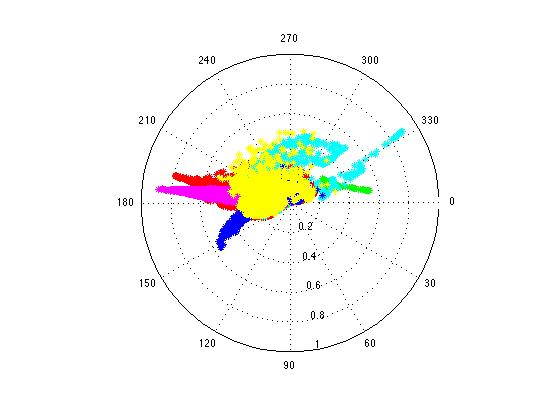
\includegraphics[width=0.33\textwidth]{figures/new_results/without_normalisation/Ses01F_impro01_gamma_emo.jpg}
}
%\\
\subfloat[All gamma emotions excluding neutral]
{
\centering
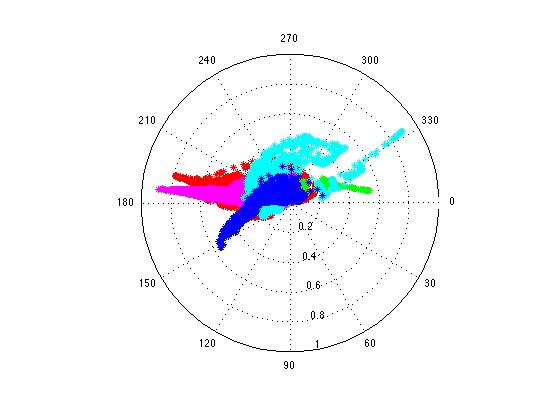
\includegraphics[width=0.33\textwidth]{figures/new_results/without_normalisation/Ses01F_impro01_gamma_emo_excluding_neu.jpg}
}
%\\
\subfloat[Gamma neutral]
{
\centering
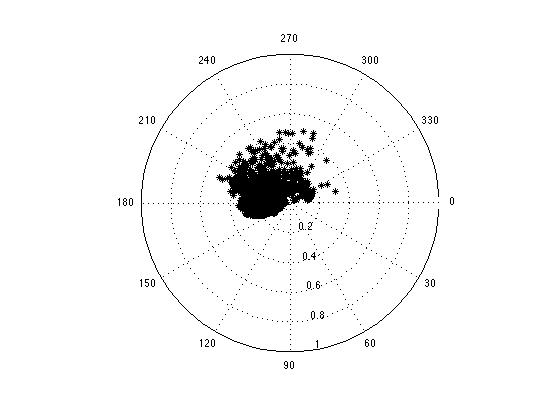
\includegraphics[width=0.33\textwidth]{figures/new_results/without_normalisation/Ses01F_impro01_gamma_neutral.jpg}
}
\end{center}
\caption{Gammas of all emotions without normalisation}
\label{fig_without_norm_depen_vs_indepen}
\end{figure*}

Explain Gamma

\section{Analysis of Emotion Dynamics}
\label{sec_analysis}
The research related to the study of `discrete emotion dynamics' focuses mainly on the detection of four temporal segments: neutral, where there is no sign of activation of any facial expression; the onset of a facial expression, when the muscular contraction begins and increases in intensity; the apex, which is the peak where the intensity reaches a stable level; and the offset, which is the relaxation of the muscular action back to the neutral state.

However, emotions are not discrete: they continuously change over time due to their natural progression, external stimuli, and the way the face works. Naturally, emotions fade in their intensity with time~\cite{ritchie2009fading}: the intense anger that might have been accompanied by betrayal by a close friend might provoke a milder response when recalled after weeks or months. Similarly, the intense feeling of joy accompanied by winning a championship might provoke a milder sense of happiness when looking at the event's photos weeks or months later. Also, research shows that a noticeable change in emotions is brought about by an external stimulus, e.g., the behaviours of others, or a change in the current situation, or internal stimuli such as thoughts or memories~\cite{scherer2000psychological}. 

In addition, emotional \emph{expressions} change based on the mechanical properties of facial skin. The facial dermal tissues comprise collagen $(72\%)$ and elastin $(4\%)$ fibres which help resist deformation of tissues. Therefore, the facial tissues effected by the active muscle activity caused by emotion expressions need to relax before stretching to another form (i.e., expressing another emotion)~\cite{terzopoulos1990physically}. Moreover, emotions are related to each other in a systematic manner which guides the way emotions go through transition from one state to another. For example, the transition from anger to frustration is more common than the transition from anger to happiness.

So far, none of the computational studies have focused on the temporal analysis of `continuous emotions dynamics' in order to understand the relationships between different emotions and the paths followed by emotions while moving from one state to another (i.e., emotion trajectories).

This paper addresses these problems by taking into account continuous spontaneous expressions of emotions. It focuses on the study of complex emotions as the weighted set of basic emotions, considering their relationships with each other. In addition, this paper presents ways to study the temporal dynamics of continuous emotions in order to get insight about the emotion trajectories and the corresponding intensity variations over time.

\begin{figure}[!t]
\centering
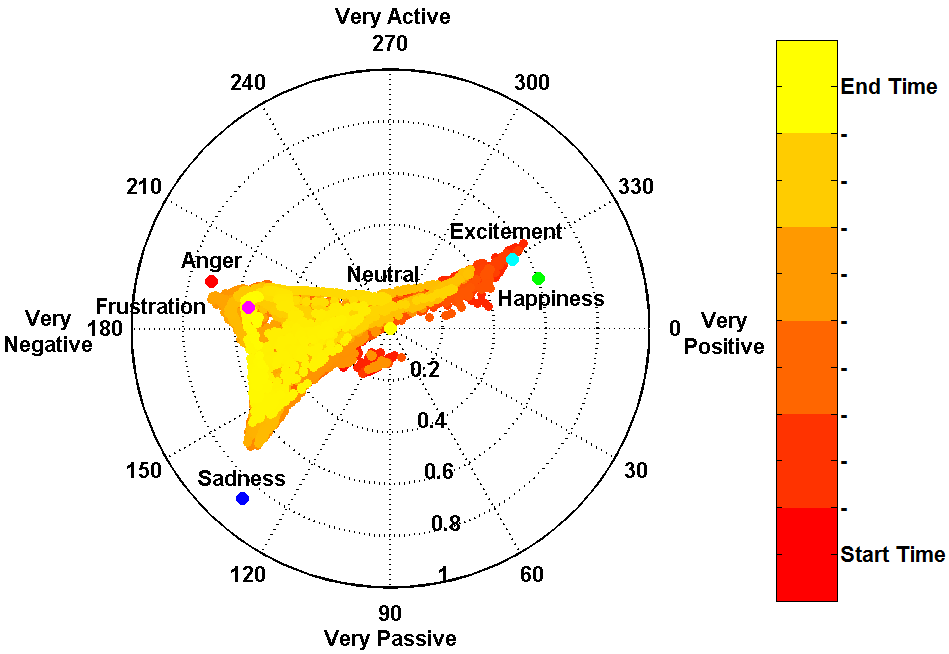
\includegraphics[width=0.5\textwidth]{figures/Ch7/con_emo_traj_color_up.png}
\caption{The mapping of continuous emotions during a conversation (Ses01F$\_$impro01) into the activation-evaluation space. The movement of emotions through time is represented by changing colour spectrum from dark/red (start) to light/yellow (end).}
\label{fig_con_emo_traj_color_up}
\end{figure}


% Edit the figure name and give this description in the results section

The paths of emotional expressions are observed in the activation-evaluation space. Fig.~\ref{fig_con_emo_traj_color_up} shows the mapping of continuous emotions through time corresponding to an unsegmented conversation in the activation-evaluation space (using the methods described in Section~\ref{sec_methodology}). The colour variation represents time, ranging from red (dark in grayscale) to yellow (light in grayscale). The figure shows some sequence information in the transition from one emotion state to another. Also, we already knew the mechanical properties of facial dermal tissues and that the emotions are related to each other in a systematic manner, as discussed in Section~\ref{sec:introduction}. All these facts and findings motivated us to computationally analyse the paths of emotions while transitioning from one state to another. We propose the following hypotheses about the emotion paths representation in the activation-evaluation space:

\begin{enumerate}
\item The paths among emotions form `smooth' trajectories in the space.
\item If the end-point emotions are not positively correlated, then the path goes through the neutral state.
\item If the end-point emotions are positively correlated, then the path does not go through the neutral state.
\end{enumerate}

Positively correlated emotions are those that lie close to each other (less than $90\degree$ divergence) in the activation-evaluation space. Uncorrelated emotions correspond to the emotions that lie at $90\degree$ divergence, while the negatively correlated emotions corresponds to the emotions which are $180\degree$ apart in the activation-evaluation space. 

\subsection{Evaluation}
\label{sec_evaluation}

Within the following section the methods used to test the proposed hypotheses are presented, together with the results of those tests.

\paragraph*{Hypothesis 1: The paths among emotions form `smooth' trajectories in the space.}
\label{para_hypothesis_1}

In order to test the first hypothesis,  we first need to define `smoothness' of an emotion trajectory. After extensive review of the literature, we could not find any standard definition. However, if we consider an emotion trajectory as a time series (sequence of values at successive time points following a non-random order), then its smoothness may be defined as a measure of its persistence with time. A random time series, e.g., Brownian motion, is not smooth, as it is not persistent with time. On the basis of this definition, we may say that if the points in the emotion space move in a predictable manner then the resulting trajectory is smooth/persistent with time.

We measure the smoothness of emotion points trajectories in the activation-evaluation space using two approaches: \emph{first}, by measuring the time derivative of angular displacement (angular velocity) and \emph{second}, by estimating the Hurst exponent ($H$)~\cite{qian2004hurst}. The time derivative of angular displacement determines the change in the angle with time; the smaller the change, the smoother the trajectory and vice-versa. It is approximated by:

\begin{center}
$\dot{\theta_{t}}=\theta_{t}-\theta_{t-1}$  \\
\end{center}

\noindent where $t=2,3,\cdots,n$ and $n=$ total number of frames in the video. We plotted the time derivatives of angular displacement of the emotion points during each conversation in the testing set and got smaller values that imply smooth emotion trajectories~\cite{ayesha hakim analysis paper}.

The Hurst exponent is a statistical measure of persistence and predictability of a time series, calculated by rescaled range $\left(\frac{R_{t}}{S_{t}}\right)$ analysis, where $R_{t}$ is the rescaled range and $S_{t}$ is the standard deviation of the time series. The calculation of the rescaled range $R_{t}$ of the time series will be described shortly. The greater the value of $H$ $(0.5<H<1)$, the smoother the time series, $H=0.5$ means a random time series. We plotted the the Hurst exponent as a measure of smoothness of emotion trajectories in the activation-evaluation space for each conversation in the testing set and got all values close to $1$~\cite{ayesha hakim analysis paper}. We estimated $H$ for the time series representing the size of `change' between pairs of consecutive points in the space as a function of valence and activation. Suppose $X_{t}$ denotes the time series where $t=2,3,\cdots,n$ and $n=$ total number of frames in the video. The size of `change' for each frame is calculated as the Euclidean distance between the time derivative of valence $(\dot{V_{t}})$ and the time derivative of activation $(\dot{A_{t}})$ in the activation-evaluation space:

\begin{center}
$\dot{V_{t}}= V_{t}-V_{t-1} $  \\
$\dot{A_{t}}= A_{t}-A_{t-1} $ \\
\end{center}

\noindent where the $t$ index represents the $t^{th}$ element of the time series.

\begin{equation}
\label{eq_size_of_change}
\text{size of change}=\sqrt{\dot{V_{t}}^{2}+\dot{A_{t}}^{2}}
\end{equation}

\noindent The rescaled range $R_{t}$ of time series $(X_{t})$ is calculated by:

\begin{enumerate}
\item Calculate the mean-centred time series $Y_{t}=X_{t}-\mu$, where $\mu$ is the mean of the time series.
\item Calculate the cumulative sum of $Y_{t}$,
\begin{center}
$Z_{t}=\sum \limits_{i=1}^t Y_{i}$
\end{center}
\item Calculate the rescaled range $R_{t}$ of time series,
\begin{center}
$R_{t}=\max(Z_{1}, Z_{2}, \cdots, Z_{t}) - \min(Z_{1}, Z_{2}, \cdots, Z_{t})$
\end{center}
\end{enumerate}

\noindent $S_{t}$ is the standard deviation of the time series. The ratio $\frac{R_{t}}{S_{t}}$ scales as a power law with time so that:
\begin{center}
%$\left(\frac{R}{S}\right)_{t}=c \times t^{H}$ \\
$H=\frac{\log \left( \left( \frac{R}{S} \right) _{t} \right) - c}{\log(t)}$
\end{center}
\noindent where $c$ is a constant and the slope of the regression line ($R/S$ versus $t$ in log-log axes) approximates the Hurst exponent. Figure~\ref{fig_hurst_slope} shows the linear regression model fitted to the $R/S$ analysis of all emotion trajectories in the testing set.

\begin{figure}[!htp]
\centering
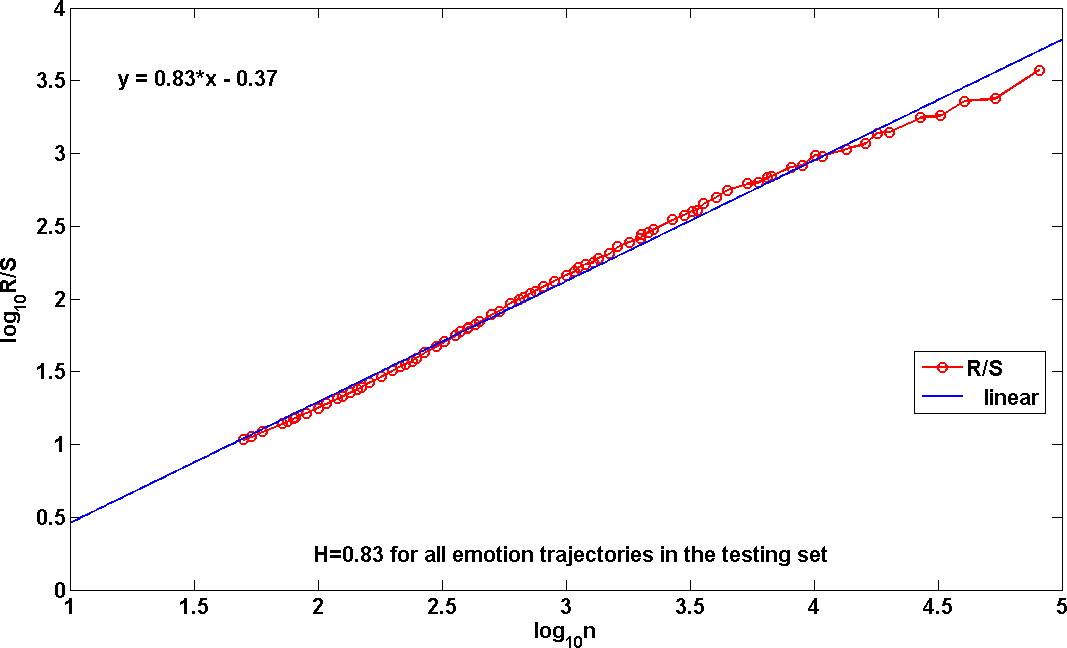
\includegraphics[width=0.5\textwidth]{figures/Ch7/hurst_slope.png}
\caption{A linear regression model fitted to $R/S$ analysis for all emotion trajectories in the testing set.}
\label{fig_hurst_slope}
\end{figure}

We calculated the size of `change' between two consecutive emotion points in the activation-evaluation space for each conversation in the testing set separately and found that the size of `change' (which is the motion within $120^{th}$ of a second) is mostly very small. However, in a few cases the size of change is bigger. In order to find the reason behind these intensity jumps (those beyond the first standard deviation), we monitored those paths of trajectories and compared them with the original videos in the dataset. We noticed that the bigger size of change in the trajectories are  false positives due to closing the eyes. We had tried to avoid this by removing the eyelid markers, but still the closing of eyes is captured by the muscles around the eyes, especially those near the eyebrows. Fig.~\ref{fig_false_pos} shows some of the false positives during transition from excitement to frustration. As lowering eyelids/eyebrows is one of the expressions of sadness, the outliers in the emotion space lies in the direction of sadness. It should be noted that the size of `change' refers to the size of displacement between the two consecutive points in the activation-evaluations space, not the displacement of markers on the face.

\begin{figure}[!ht]
\centering
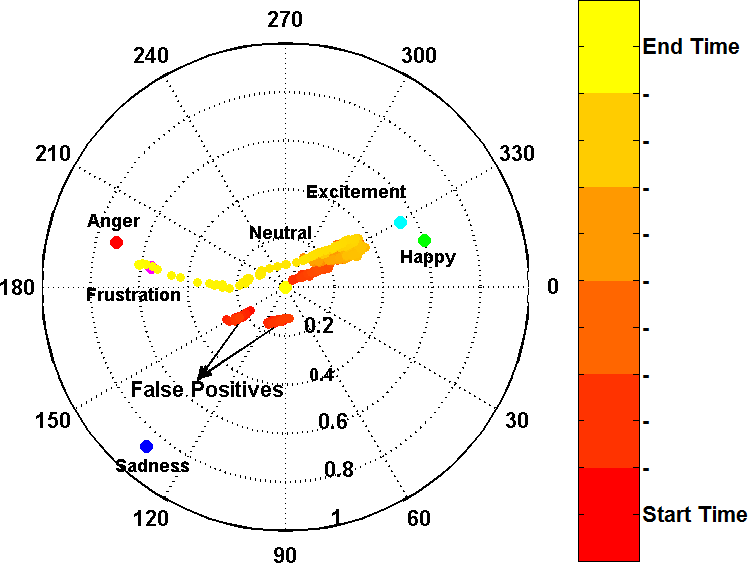
\includegraphics[width=0.5\textwidth]{figures/Ch7/false_pos_color.png}
\caption{The false positives appear during transition from neutral to excited. The movement of emotions through time is represented by changing colour spectrum from dark/red (start) to light/yellow (end).}
\label{fig_false_pos}
\end{figure}

\paragraph*{Hypotheses 2 and 3: Transitions between uncorrelated or negatively correlated emotions need to pass through the neutral state, while transitions between positively correlated emotions do not.}
\label{para_hypothesis_2_3}

According to differential emotion theory, each discrete emotion is related to certain other discrete emotions with a distinct pattern~\cite{blumberg1991patterns}. In the activation-evaluation space, emotions lie along particular angles on the basis of their similarity measures.

% Update the figure name

While looking at  continuous trajectories in the activation-evaluation space (e.g., Fig.~\ref{fig_con_emo_traj_color_up}), we noticed some patterns of emotion transitions. We fitted regression lines to the trajectories among six emotions (neutral, happiness, excitement, anger, frustration, and sadness). There are 15 possible symmetric paths among the six emotions, but the regression analysis shows that actually only seven paths are represented for all possible transitions among these emotions. For instance, the \emph{smiling} expression (getting happy) shows a linear relationship of valence and activation between neutral and happiness. The onset of smiling occurs at neutral, reaches apex at some intensity of happiness and returns to neutral for offset. In the case of \emph{laughing}, which is another expression of happiness, the same pattern repeats several times depends on its duration and intensity.

\begin{figure*}[!htp]
\begin{center}
\subfloat[Continuous transition between excitement and frustration, which are negatively correlated emotions]
{
\centering
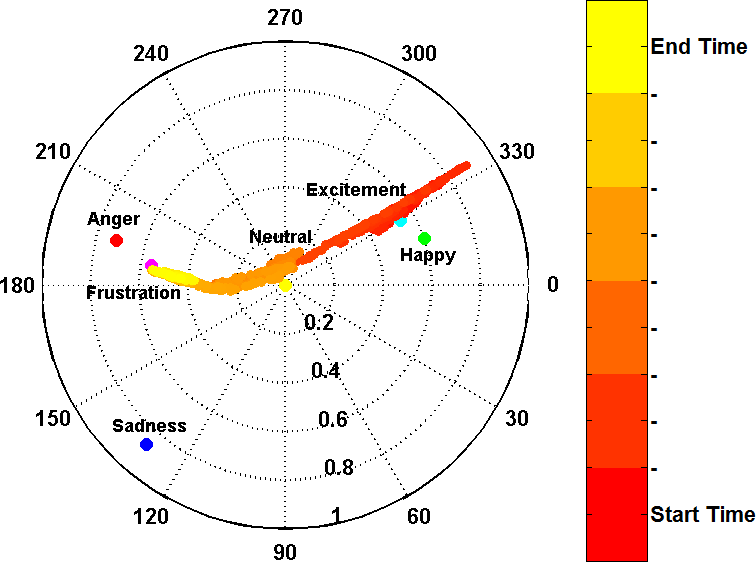
\includegraphics[width=0.5\textwidth]{figures/Ch7/exc_fru_color.png}
}
%\\
\subfloat[Continuous transition between anger and frustration, which are positively correlated emotions]
{
\centering
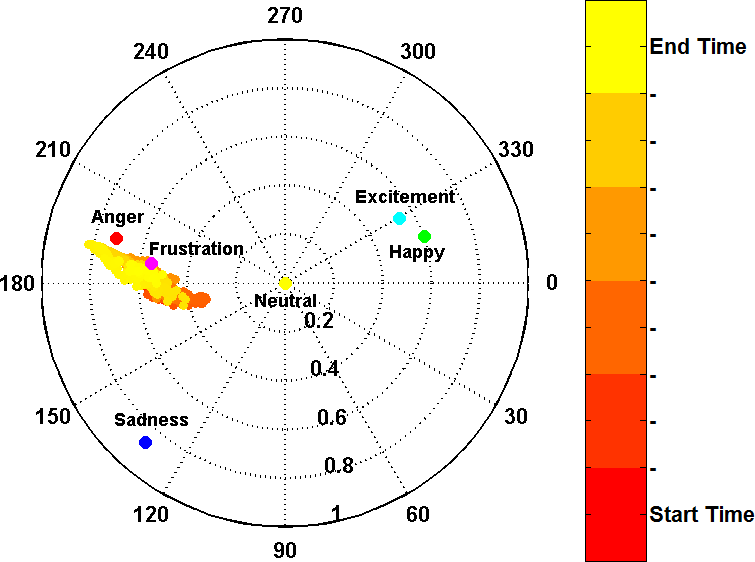
\includegraphics[width=0.5\textwidth]{figures/Ch7/ang_fru_color.png}
}
\end{center}
\caption{Transitions between negatively correlated emotions tend to pass through the neutral state, while transitions between positively correlated emotions do not.}
\label{fig_e1_to_e2}
\end{figure*}

By observing the trajectories between two uncorrelated and negatively correlated emotional states, we found that the transition between these states tends to pass through the neutral state. The intensity of the current emotion must decrease to neutral (shown as linear motion along a radial line) before the intensity of the next emotion increases. Fig.~\ref{fig_e1_to_e2}(a) shows a trajectory followed by the transition from excitement to frustration. However, the positively correlated emotions (such as anger and frustration, as well as happiness and excitement) may move from one state to another with slight change in intensity and angle simultaneously, as shown in Fig.~\ref{fig_e1_to_e2}(b). These findings are also supported by the mechanical properties of facial dermal tissues~\cite{terzopoulos1990physically}. Under low stress (transition between two positively correlated emotions), dermal tissue applies low resistance to stretch as the collagen fibres uncoil in the direction of the strain. However, under high stress conditions (transition between two negatively or uncorrelated emotions), the elastin fibres behave like elastic springs to return the collagen fibres to their original no-stress condition. According to these properties, to express a very different emotion the facial muscles have to pass through a `no-stress' condition.

\begin{table}[ht!]
\centering
\begin{tabular}{|p{3cm}|>{\centering\arraybackslash}p{1.2cm}| >{\centering\arraybackslash}p{1.2cm}|>{\centering\arraybackslash}p{1.2cm}|}
\hline
\textbf{Emotion Transition} & \textbf{Linear $(R^{2})$} & \textbf{Quadratic $(R^{2})$} & \textbf{Cubic $(R^{2})$} 
\\
\hline
Neutral-Anger & 0.9131 &  0.9297 & 0.9139
\\
\hline
Neutral-Frustration & 0.9642 & 0.9854 & 0.9924
\\
\hline
Neutral-Happiness & 0.9223 & 0.9323 & 0.9418
\\
\hline
Neutral-Excitement &  0.9374 & 0.9383 & 0.9388
\\
\hline
Neutral-Sadness & 0.902 &  0.9144 & 0.9164
\\
\hline
Anger-Frustration & 0.0922 & 0.6494 & 0.6497
\\
\hline
Happiness-Excitement & 0.0457 & 0.5914 & 0.6083
\\
\hline
\end{tabular}
\caption{Coefficient of determination $(R^{2})$ of linear, quadratic, and cubic polynomial regression models fitted to the seven symmetric paths of emotion transitions into the activation-evaluation space.}
\label{table_models}
\end{table}

Table~\ref{table_models} shows a comparison among the coefficient of determination $(R^{2})$ of linear, quadratic, and cubic polynomial regression models fitted to each of the seven symmetric paths (i.e., between neutral and happiness, neutral and excitement, neutral and anger, neutral and frustration, neutral and sadness, anger and frustration, and happiness and excitement). For the paths from neutral to any of the five emotions, there is no significant difference between the $(R^{2})$ values of linear, quadratic and cubic regression, which implies that a linear model may be used to fit these paths. For the path between neighbouring emotions such as anger to frustration as well as happiness to excitement, the quadratic regression is significantly better than the linear regression. Moreover, there is no significant difference between quadratic and cubic regressions, which implies that quadratic model may be used to fit the trajectories between the neighbouring emotions onto the activation-evaluation space.




In the activation-evaluation space, the travel along the emotion flows/trajectories is a matter of intensity change and the angle change. As already discussed, the emotion trajectories follow `common' paths, which in turn suggests that there exists some relationship between the intensity change and angle change through time. In order to analyse this relationship, we plot the polar coordinates ($\dot{r}$: changing intensity, $\dot{\theta}$: changing emotion) of continuous points in the space during emotion transitions. Fig.~\ref{fig_controlchart} consists of four subplots showing $r$ and $\theta$ respectively. In these plots, the three horizontal lines represent the mean $(\mu)$ and mean $\pm$ 1 standard deviation $\sigma$. The third and fourth subplots show change versus no-change using a binary plot by applying the following rules to the time derivatives $(\dot{r_{t}},\dot{\theta_{t}})$ of $(r,\theta)$ respectively (where the $t$ index represents the $t^{th}$ element of the time series):

\begin{center}
$f(\dot{\theta_{t}}) = \left\{ \begin{array}{ll}
0, 	&	 \text{if } \mu_{\dot{\theta_{t}}}-\sigma_{\dot{\theta_{t}}}<\dot{\theta_{t}}<\mu_{\dot{\theta_{t}}}+\sigma_{\dot{\theta_{t}}} \\ 
1, 	&	 \text{otherwise}
\end{array}\right.$ \\
$f(\dot{r_{t}}) = \left\{ \begin{array}{ll}
0, 	&	 \text{if } \mu_{\dot{r_{t}}}-2\sigma_{\dot{r_{t}}}<\dot{r_{t}}<\mu_{\dot{r_{t}}}+2\sigma_{\dot{r_{t}}} \\ 
1, 	&	 \text{otherwise}
\end{array}\right.$
\end{center}

Fig.~\ref{fig_controlchart} shows that there is a relationship between angle change and intensity change such that whenever there is a large `change' in angle (according to the given rules), the intensity decreases.

\begin{figure*}[!t]
\begin{center}
{
\centering
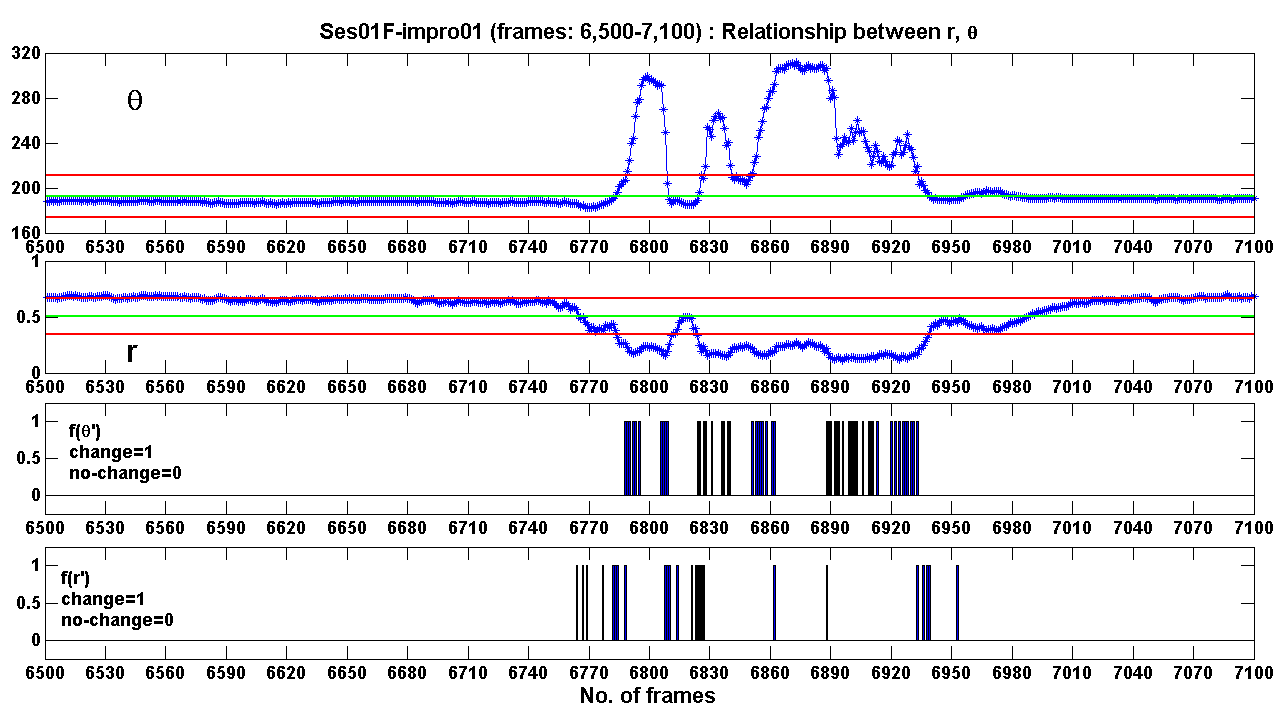
\includegraphics[width=1\textwidth]{figures/Ch7/6750_6950_change_1.png}
}
\end{center}
\caption{Ses01F$\_$impro01, continuous frames during emotion transition from anger to happiness. The temporal relationship between intensity change and angle change can be seen in the frames from 6750 to 6950. For explanation, see the text.}
\label{fig_controlchart}
\end{figure*}

\section{Discussion}
\label{sec_discussion}

This paper has presented our approach to map facial points to an appropriate emotion-space to analyse the paths of emotions while moving from one state to another. We develop a shape model for both speaker-dependent and speaker-independent discrete emotion recognition. It give us the distance of each frame from five emotion states and the neutral state. We perform speaker-reference based normalisation to minimise the effect of speaker-face variability. We compared the results of our system with the majority label out of more than three labels assigned by three human evaluators and the speaker-independent model gives highest recognition accuracy after reference-based normalisation.

The research in psychology has shown that in everyday interactions people exhibit non-basic, intermediate, or complex emotional states which are related to each other in a systematic manner. Based on this, it is not appropriate to assign a single independent categorical label to complex emotions which are mixtures of more than one emotion category. Also, sometimes the difference between two or more emotions is so subtle that it becomes difficult to finely differentiate between them. Due to this ambiguity, human evaluators assigned more than one categorical label to each turn.

Motivated by these thoughts, in this paper we address the problem of spontaneous complex emotion recognition by mapping them into the emotion space. Instead of classifying the emotions to one emotion category based on the best-matched criteria, we add the effect of all basic emotions for the recognition of complex emotions. 

Using the von Mises mixture model, we presented a technique for the recognition and representation of complex emotions in the activation-evaluation space. The proposed method is based on the psychological assumption that complex emotions are comprised of mixtures of basic emotions. There is still debate among psychologists on the number of basic emotions and which emotions should be considered as basic, and of the six emotions that we have considered two (frustration and excitement) are candidate basic emotions. However, the proposed mixture model is quite flexible and can be applied to any set of basic emotions. We estimated the degree of similarity of each test frame to each of the basic emotions and project them into the activation-evaluation space using the von Mises mixture model.

Using von Mises mixture model, each continuous conversation is mapped into the activation-evaluation space frame by frame. However, we know that emotions are related to each other in a systematic manner which guides the way emotions go through transition from one state to another~\cite{blumberg1991patterns}. In order to understand the relationships among different emotions and the paths followed by emotions while moving from one state to another (i.e., emotion trajectories), we extended this work to the computational analysis of continuous emotion trajectories in the activation-evaluation space~\ref{sec_analysis}. Emotions vary in intensity, flow, persistence with time, and their relationships with other emotions. By analysing the emotion dynamics through time, we try to seek the answers about the `common' paths between emotions, the smoothness of emotion trajectories, and how we travel along emotion flows. The computational analysis of emotion dynamics may be helpful for better understanding of emotion trajectories as well as in the development of more flexible models for emotion recognition, representation, and synthesis.

Section~\ref{sec_analysis} presented an analysis of emotion trajectories in the activation-evaluation space based on shape models of facial points. On the basis of trajectory-level analysis, we evaluated some hypotheses related to the smoothness of emotion trajectories, and the `common' paths among emotions based on their correlation.

By measuring the size of `change' between two consecutive frames, we found that the emotions move in a continuous flow, which implies that there are no sudden jumps within the trajectories. Further, we measured the smoothness of continuous emotion trajectories on the basis of the time derivative of angular displacement and the estimated Hurst exponent, which suggests that the emotion trajectories are smooth and persistent with time.

By visualising the emotion trajectories, we observed that there are 15 possible symmetric paths among the six emotions in the activation-evaluation space. To test it, we fitted regression lines to the trajectories and found that there are actually only 9 symmetric paths to travel among these six emotions. We showed that a linear model fits well to the trajectories between neutral and any of the other five emotions. The trajectories between uncorrelated and negatively correlated emotions cannot be fitted with one linear model, however, two linear models are better fitted than one quadratic or cubic regression model. A quadratic regression model fits well to the trajectories between positively correlated emotions. 

By analysing the relationship between the change in angle and change in intensity, we may conclude that the transition between negatively correlated or uncorrelated emotions causes a decrease in intensity, while the transition between positively correlated emotions may occur with a slight change in intensity and angle simultaneously. 

The presented analysis might be used and extended in several directions, such as examining the `abnormal' paths of emotions, which might give some cues about underlying deception, or some illness. The mapping of continuous trajectories to the activation-evaluation space might be a useful tool to build emotional conversation agents displaying realistic emotions and going through smooth emotion transitions.

\section*{Acknowledgments}
This work was supported by funds from the Higher Education Commission (HEC) Pakistan. The authors would like to thank Massey University for providing support throughout the research.

%This paper is an extension of the paper "A Robust Joint Face Model for Human Emotion Recognition"~\cite{hakim12} published in IVCNZ, 2013.

\ifCLASSOPTIONcaptionsoff
  \newpage
\fi
% trigger a \newpage just before the given reference
% number - used to balance the columns on the last page
% adjust value as needed - may need to be readjusted if
% the document is modified later
%\IEEEtriggeratref{8}
% The "triggered" command can be changed if desired:
%\IEEEtriggercmd{\enlargethispage{-5in}}

% references section


\bibliographystyle{IEEEtran}
\bibliography{bib_computational_modelling} 

%\begingroup
%\fontsize{9}{9}\selectfont
\begin{biography}[{
\includegraphics[width=1in,height=1.25in,clip,keepaspectratio]{AHM.jpg}}]{Ayesha Hakim}

Ayesha Hakim has a BS(Hons.) in Computer Science from Bahauddin Zakariya University, Multan, Pakistan, which she completed in 2006. She received a gold medal for reaching the first position in the university and obtaining the highest CGPA record. She worked as Assistant Professor of IT in the same university. Along with the lectureship, she spent time working as a software engineer in a multinational company. On the basis of her excellant academic background, the Higher Education Commission of Pakistan granted her the Indigenous Scholarship to complete a doctrate in computer science. She joined Massey University in July 2008, where she completed her PhD in 2014. Her research interests include affective computing, human-computer interaction, mobile computing, and context-aware systems.
\end{biography}

\begin{biography}[{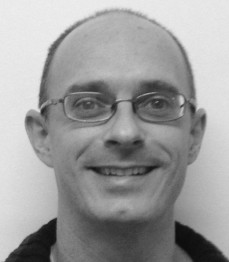
\includegraphics[width=1in,height=1.25in,clip,keepaspectratio]{SRM.jpg}}]{Stephen Marsland}

Stephen Marsland has a BA(Hons) in Mathematics from the University of Oxford and a PhD in "Self-Organisation and Novelty Detection" from the University of Manchester, which he completed in 2002. Since then he has spent time at the Santa Fe Institute, the University of Bremen and the University of Manchester, where he was a lecturer in computer science and a researcher in the divison of Imaging Science and Biomedical Engineering. He moved to Massey University in 2004, and was awarded an Early Career research award there in 2005. He is currently a professor and the postgraduate director of the School of Engineering and Advanced Technology at Massey University.
\end{biography}

\begin{biography}[{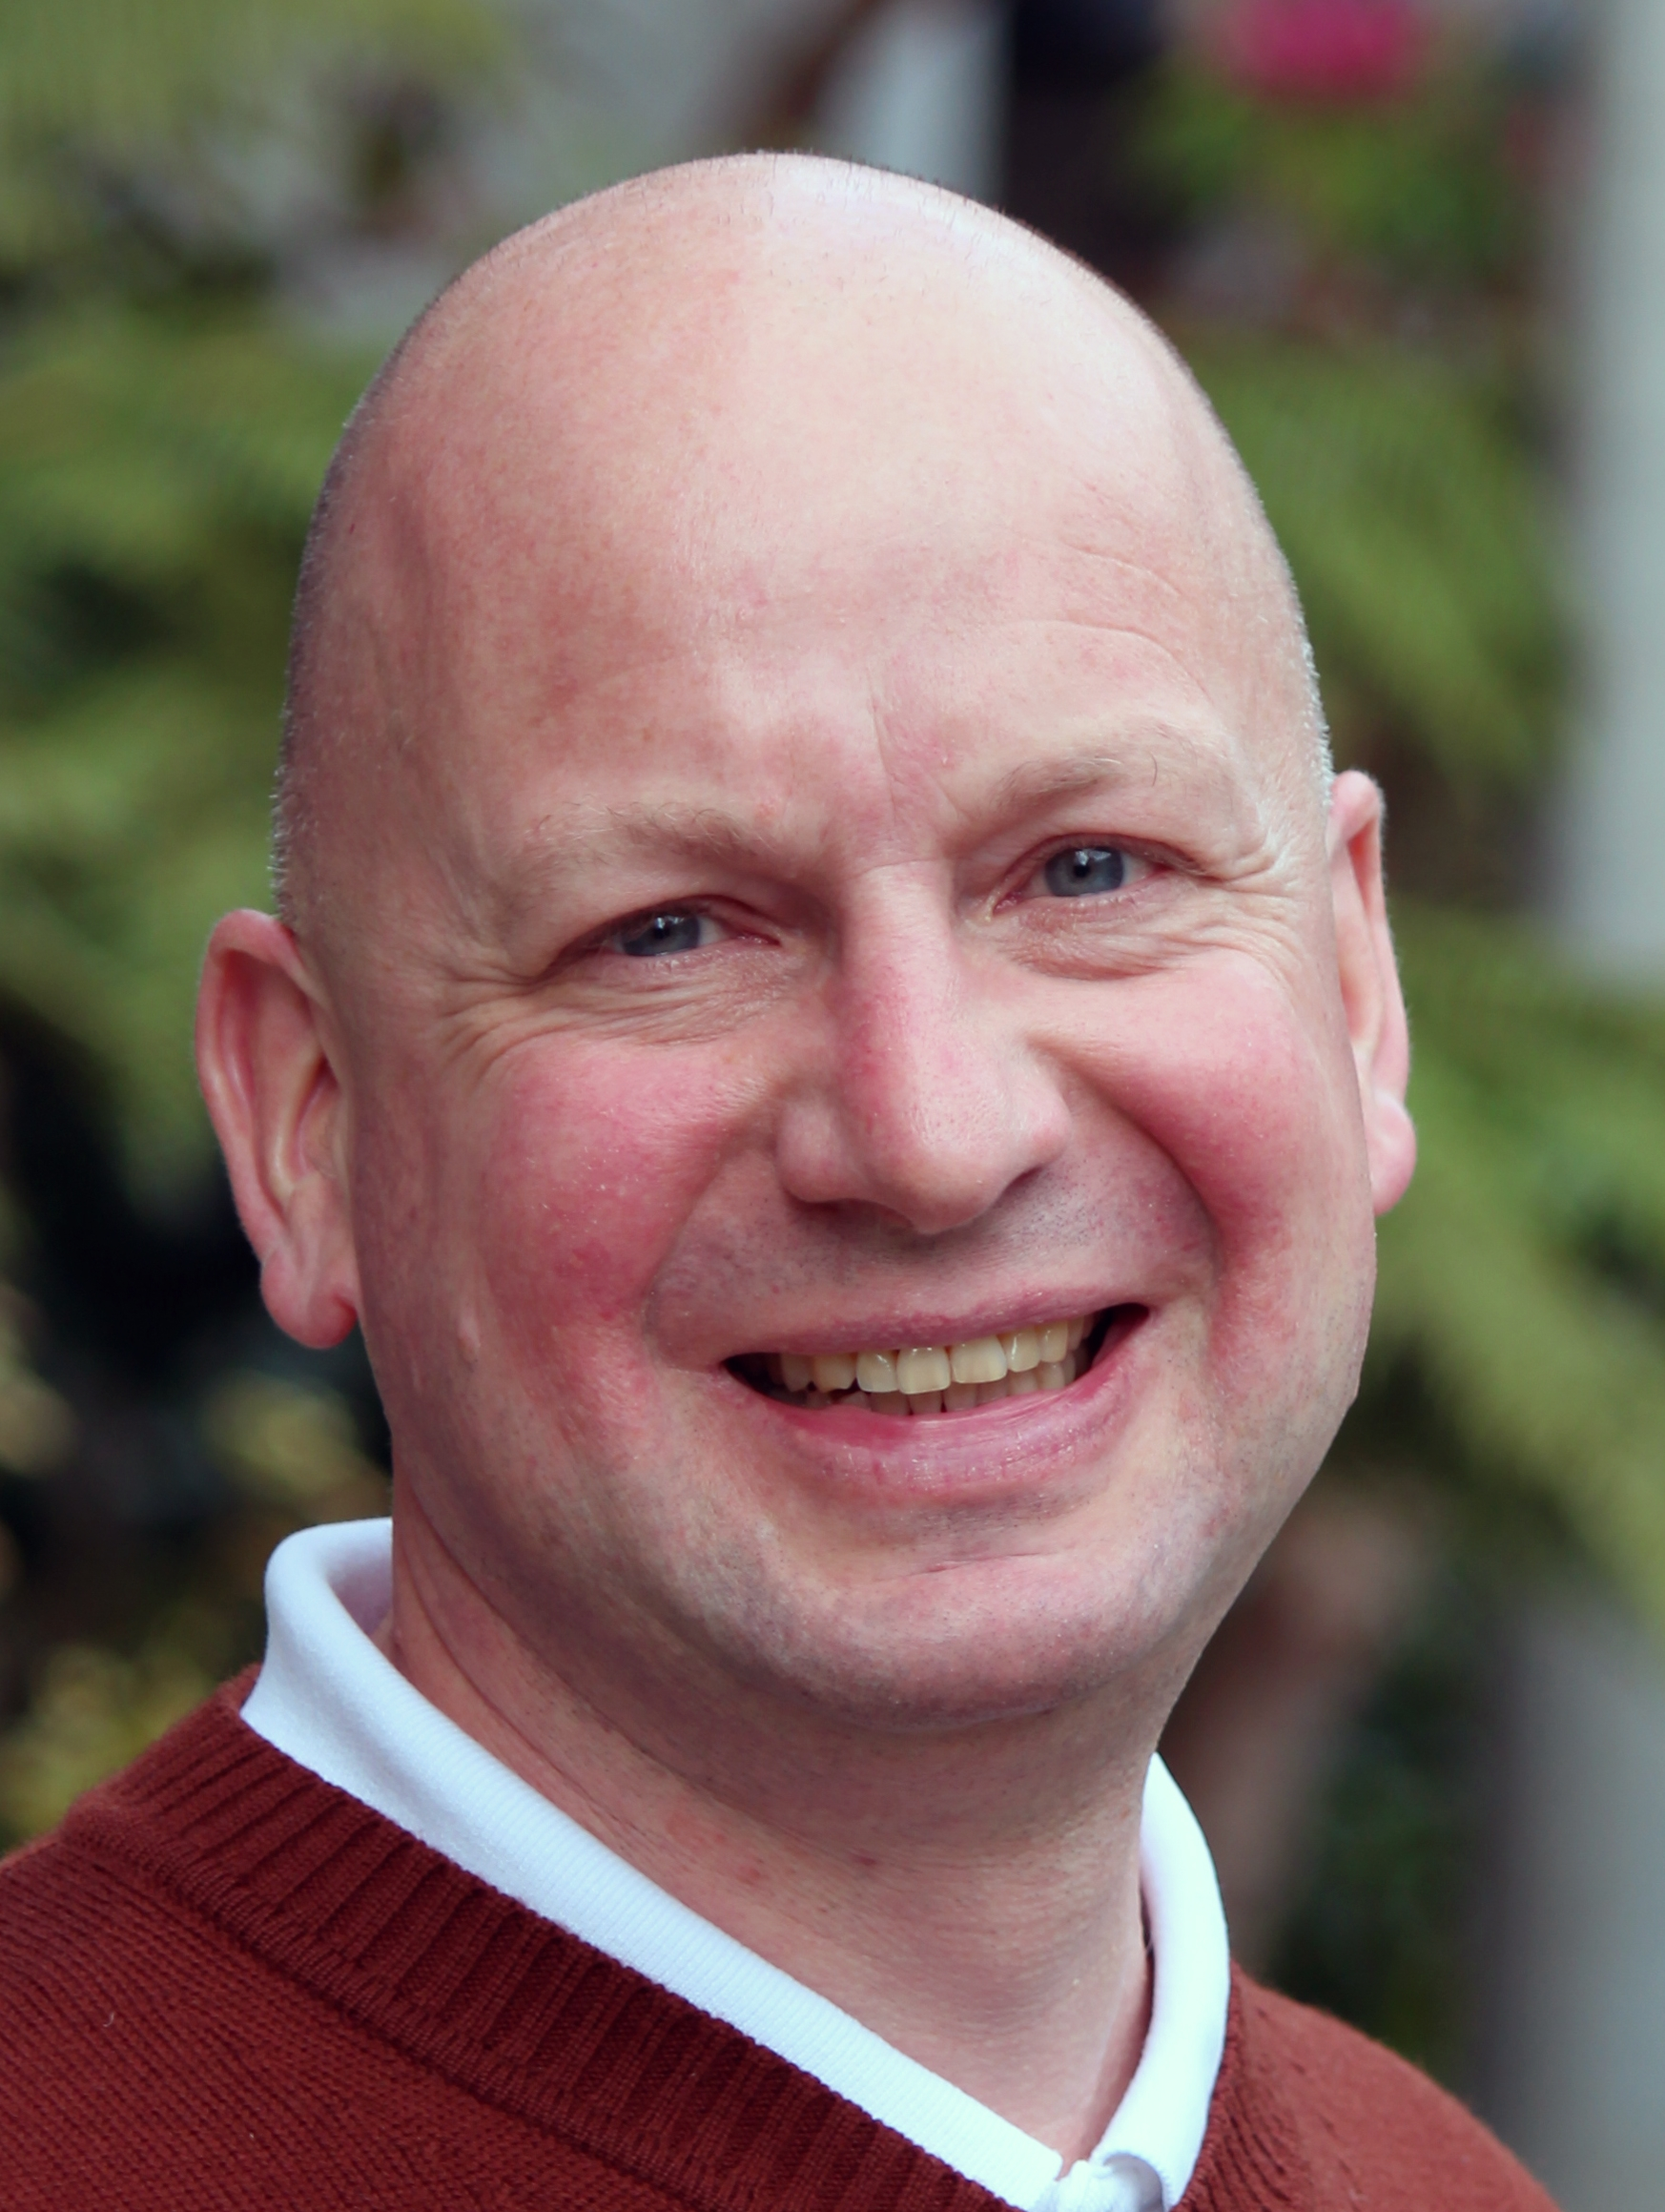
\includegraphics[width=1in,height=1.25in,clip,keepaspectratio]{HWG.jpg}}]{Hans W. Guesgen}

Hans Guesgen holds a diploma in computer science and mathematics of the University of Bonn, a doctorate in computer science of the University of Kaiserslautern, and a higher doctorate (Habilitation) in computer science of the University of Hamburg, Germany. He worked as a research scientist at the GMD in Sankt Augustin from 1983 to 1992, primarily in the area of artificial intelligence and expert systems. 
%During this period he held a one-year post-doctoral fellowship at the International Computer Science Institute in Berkeley, California, where his research focus changed to spatial and temporal reasoning. 
In 1992 he joined the Computer Science Department of the University of Auckland, where for almost fifteen years he led the AI research group. % and was involved in projects on constraint satisfaction, spatio-temporal reasoning, fuzzy logic, heuristic search, computer games, health informatics and others. 
In 2007, he was appointed Chair of Computer Science in the School of Engineering and Advanced Technology at Massey University.
\end{biography}
%\endgroup

% if you will not have a photo at all:
%\begin{IEEEbiographynophoto}{Stephen Marsland}
%Biography text here.
%\end{IEEEbiographynophoto}

% insert where needed to balance the two columns on the last page with
% biographies
%\newpage

%\begin{IEEEbiographynophoto}{Hans W. Guesgen}
%Biography text here.
%\end{IEEEbiographynophoto}

% You can push biographies down or up by placing
% a \vfill before or after them. The appropriate
% use of \vfill depends on what kind of text is
% on the last page and whether or not the columns
% are being equalized.

%\vfill

% Can be used to pull up biographies so that the bottom of the last one
% is flush with the other column.
%\enlargethispage{-5in}



% that's all folks
\end{document}